% arara: pdflatex: { synctex: yes }
% arara: makeindex: { style: ctuthesis }
% arara: bibtex

% The class takes all the key=value arguments that \ctusetup does,
% and a couple more: draft and oneside
\PassOptionsToPackage{table}{xcolor} % avoid clash with \usepackage[table]{xcolor}
\documentclass[twoside]{ctuthesis}

\ctusetup{
%	preprint = \ctuverlog,
%	mainlanguage = english,
%	titlelanguage = czech,
    mainlanguage = english,
	otherlanguages = {czech},
	title-czech = {Vizuální lokalizace pro HoloLens},
	title-english = {Visual Localization with HoloLens},
	%subtitle-czech = {Cesta do tajů kdovíčeho},
	%subtitle-english = {Journey to the who-knows-what wondeland},
	doctype = M,
	faculty = F3,
	department-czech = {Katedra počítačů},
	department-english = {Department of Computer Science},
	author = {Pavel Lučivňák},
	supervisor = {doc. Ing. Tomáš Pajdla Ph.D.},
	supervisor-address = {CIIRC ČVUT, \\ Jugoslávských partyzánů 1580/3, \\ Praha 6 - Dejvice, \\ 160 00},
	%supervisor-specialist = {TODO: kdo to je?},
	fieldofstudy-english = {Artificial Intelligence},
	subfieldofstudy-english = {Open Informatics},
	fieldofstudy-czech = {Umělá inteligence},
	subfieldofstudy-czech = {Otevřená informatika},
	keywords-czech = {HoloLens, lokalizace, Matterport, Vicon},
	keywords-english = {HoloLens, localization, Matterport, Vicon},
	day = 14,
	month = 8,
	year = 2020,
	specification-file = {Lucivnak-Zadani-DP.pdf},
	front-specification = true,
%	front-list-of-figures = false,
%	front-list-of-tables = false,
%	monochrome = true,
%	layout-short = true,
}

\ctuprocess

\addto\ctucaptionsczech{%
	\def\supervisorname{Vedoucí}%
	\def\subfieldofstudyname{Studijní program}%
}

\ctutemplateset{maketitle twocolumn default}{
	\begin{twocolumnfrontmatterpage}
		\ctutemplate{twocolumn.thanks}
		\ctutemplate{twocolumn.declaration}
		\ctutemplate{twocolumn.abstract.in.titlelanguage}
		\ctutemplate{twocolumn.abstract.in.secondlanguage}
		\ctutemplate{twocolumn.tableofcontents}
		\ctutemplate{twocolumn.listoffigures}
	\end{twocolumnfrontmatterpage}
}

% Theorem declarations, this is the reasonable default, anybody can do what they wish.
% If you prefer theorems in italics rather than slanted, use \theoremstyle{plainit}
\theoremstyle{plain}
\newtheorem{theorem}{Theorem}[chapter]
\newtheorem{corollary}[theorem]{Corollary}
\newtheorem{lemma}[theorem]{Lemma}
\newtheorem{proposition}[theorem]{Proposition}

\theoremstyle{definition}
\newtheorem{definition}[theorem]{Definition}
\newtheorem{example}[theorem]{Example}
\newtheorem{conjecture}[theorem]{Conjecture}

\theoremstyle{note}
\newtheorem*{remark*}{Remark}
\newtheorem{remark}[theorem]{Remark}

\setlength{\parskip}{5ex plus 0.2ex minus 0.2ex}

% Custom constants and macros
\usepackage{xifthen}
\newcommand{\todo}[1][]{%
\ifthenelse{\isempty{#1}}{{\color{red}{TODO}}}{{\color{red}{TODO: #1}}}%
}

\newcommand{\code}[1]{{\ttfamily #1%
}}

\newcommand{\TP}[1]{{\color{blue}#1}}

\DeclareMathOperator*{\argmin}{arg\,min}
\hyphenation{Multi-Camera-Pose}

\newcommand{\topRetrieval}{100} % ht_retrieval output
\newcommand{\topGV}{10} % number of cutout candidates for each query
\newcommand{\topPE}{10} % PE output (number of candidate poses for each query)
\newcommand{\topPV}{1} % obviously
\newcommand{\HLvsRefPosesErrorsCaption}{Estimate of reference vs ground truth poses errors. All the queries in the sequence were considered, with two kinds of exceptions. Queries, for which we do not have a reference pose (Vicon got lost) are not considered in the statistics. Queries for which we do not have a corresponding pose from HoloLens (due to the delay) are also not included in the statistics. Ground truth poses are estimated from the poses provided from HoloLens, after conversion to World coordinate system.}

% Abstract in Czech
\begin{abstract-czech}
Vizuální lokalizace je často řešená problematika v počítačovém vidění. Typicky chceme určit pózu (polohu a orientaci) fotoaparátu, který pořídil daný RGB snímek. Odhadnutá póza se vztahuje k nějakému námi definovanému souřadnicovému systému. Tento problém se například řeší ve smíšené realitě v HoloLens. Promítáme zde virtuální objekty to reálného prostoru. Abychom mohli udržet tyto objekty na správném místě, zatímco se uživatel brýlí pohybuje, je potřeba vědět, kde se HoloLens nachází. HoloLens jako takové umí sledovat svou vlastní pózu, ale výsledek není perfektní. Vytvořil jsem novou sadu dat, která obsahuje skeny dvou místností a tři množiny query obrázků. Dvě z nich pochází právě z HoloLens. Obsahem datové sady jsou i referenční pózy fotoaparátu (u některých zatím chybí, ale dají se v případě potřeby vygenerovat). Navrhl jsem nové algoritmy, které kombinují metodu InLoc \cite{taira2018inloc} s daty, co nám dává HoloLens. Má implementace je na sekvenčních obrázcích přesnější, než původní InLoc. Mé metody jsou ale výrazně méně přesné, než lokalizace ze samotných HoloLens. V práci shrnuji mé poznatky, proč vnikají určité chyby související s novými metodami nebo s InLocem. V budoucnu je možné na práci navázat a chyby zredukovat.
\end{abstract-czech}

% Abstract in English
\begin{abstract-english}
Visual localization is a common computer vision problem of estimation of the camera pose that took a particular RGB image. The pose is estimated relative to a certain coordinate system. One particular instance of this problem occurs in HoloLens mixed reality. In a mixed reality settings, we are projecting virtual objects into the real world environment. In order to maintain the objects as the user navigates around a room, we need to keep track of the device pose. HoloLens already does this, however there is a room for improvement. A new indoor visualization datasets, consisting of 2 rooms and 3 query sets, has been created. Two of these query sets are sequential images (from HoloLens). Reference poses are also provided (although not for all queries). We have designed new methods that aim to merge InLoc \cite{taira2018inloc} approach to indoor visual localization with the data from HoloLens. My implementation outperformed the original InLoc paper on the task of sequential localization from RGB images. However, our approach turned out to perform significantly worse than the pose estimation from HoloLens itself. I provide an overview of sources of errors in the new and InLoc methods for potential future improvement.
\end{abstract-english}

% Acknowledgements / Podekovani
\begin{thanks}
I would like to thank my family for their support and motivation; especially during the times when I was struggling to make progress. My supervisor Tomáš Pajdla was very helpful with his suggestions and leadership. Special thanks to Torsten Sattler, who took the time to clarify my questions about the use his open-source software; and Anna Zderadičková whose experience with HoloLens allowed me to capture the raw sequential data quickly.
\end{thanks}

% Declaration / Prohlaseni
\begin{declaration}
Prohlašuji, že jsem předloženou práci vypracoval samostatně, a že jsem uvedl veškerou použitou literaturu.

V Praze, \ctufield{day}.~\ctufield{month}.~\ctufield{year}
\end{declaration}

% Only for testing purposes
\listfiles
\usepackage[pagewise]{lineno}
\usepackage{lipsum,blindtext}
\usepackage{mathrsfs} % provides \mathscr used in the ridiculous examples
\usepackage{gensymb} % for \degree
\usepackage{csvsimple}
\usepackage{makecell}
\usepackage{adjustbox}
\usepackage{cellspace} % for table rows padding
\usepackage{subcaption} % for subfigures, subtables
\usepackage[normalem]{ulem} % strikethrough
\usepackage{diagbox} % split table cell into two diagonal cells
\usepackage[table]{xcolor} % alternate row colors in table
\usepackage[section]{placeins} % to help keep floats within their section
\usepackage{listings}
\usepackage{dirtree} % directory tree visualization
\usepackage{enumitem} % ability to create a. b. c. enumerations

\begin{document}

\maketitle

\chapter{TODO}

\begin{itemize}
	\item \todo[make sure the dependencies are properly cited as noted in their README]
\end{itemize}

%\part{Your Party}

\chapter{Introduction}

Visual localization is a common computer vision problem where, given an RGB image, we want to estimate the camera pose. Such a camera pose can be specified by 6 parameters - 3 of which describe its position in space and the other 3 represent its orientation in the space. In case of outdoor visual localization, the problem can be simplified by making use of GPS for approximate position localization. Visual localization is a problem that also needs to be addressed indoors, however. It has use cases in e.g. augmented and mixed reality applications. Of course, the GPS signal is unusable in a building. In this thesis, I am going to focus on indoor visual localization with HoloLens. HoloLens is a mixed reality device; providing a powerful tracking of the camera as user navigates around a room. The accuracy is already high, however the idea of this thesis is to improve it further. Imagine a use case where we place virtual objects into the mixed reality. As user navigates around the room, we need to track the pose of HoloLens in order to maintain the object placements. The indoor environment is problematic for several reasons. One of them being that there are a lot of similar areas - the same type of windows, doors, textureless walls. Furthermore, the environment can change easily as people interact with it.

The objectives of this work are as follows:

\begin{enumerate}
	\item State of the art in indoor localization must be reviewed; in particular the NetVLAD \cite{Arandjelovic16} and InLoc \cite{taira2018inloc} papers.
	\item A new indoor dataset based on the InLoc dataset \cite{taira2018inloc} shall be created. The new dataset must also contain query images that were taken in a sequence (as an user with HoloLens walks in the room).
	\item Make InLoc run on the newly created dataset, by processing the query images in non-sequential fashion.
	\item Implement an improvement that takes the HoloLens data into account. One of the improvements should include taking multiple historical camera data into account (InLoc currently only uses a single camera pose, because it does not deal with sequential data).
	\item At last, the performance of the newly implemented algorithms shall be evaluated.
\end{enumerate}

This work is organized the following way. Chapter \ref{chapter:literature-review} contains related work on the topic of indoor visual localization. Background that my software and algorithms rely on is also described. The newly acquired dataset is described in Chapter \ref{chapter:dataset}. It contains statistics of the dataset, its structure and how it was created. An implementation of the techniques described here are covered in Chapter \ref{chapter:implementation}. Note that it is only a proof-of-concept implementation, unsuitable for deployment out of the box (just as the InLoc implementation). Chapter \ref{chapter:evaluation} evaluates the newly developed methods and compares them with some baseline methods. Sources of errors are also noted. Finally, the Chapter \ref{chapter:conclusion} is a summary of this work, whether it fulfilled the assignment and possible future work.

\chapter{Literature review}
\label{chapter:literature-review}

This chapter provides a review of relevant work. It also provides a theoretical or technical background on topics we are dealing with within this thesis.

\section{InLoc}
InLoc \cite{taira2018inloc} a powerful method (state-of-the-art in 2018) for indoor visual localization. All the newly developed algorithms in this work use InLoc or its modification at its core. Not necessarily because there is no better method out there, but because it is the topic of this thesis (and the thesis supervisor is a co-author of the InLoc paper, which is beneficial for getting familiar with the method quickly). To understand the methods developed in this work better, it is useful to learn about InLoc first.

InLoc operates on top of an InLoc dataset. The dataset contains:

\begin{itemize}
	\item 256 query RGB photos,
	\item $10\,000$ cutout RGBD images,
	\item 277 reference panorama poses (determined using \cite{wijmans17rgbd}),
	\item reference query poses,
	\item query-cutout similarity matrix (known as \code{score}).
\end{itemize}

The dataset has been acquired at the Washington University in St. Louis. Five floors (at two buildings) were used to build the dataset. The InLoc method assumes existence of a 3D map. In the InLoc dataset, the 3D map was constructed using a high-end Faro 3D scanner. Each scan with that device produces an RGBD panorama image. The data from the various scans was then merged to create a single 3D model for each floor (using \cite{wijmans17rgbd}). In addition, database images, also called \emph{cutouts} were produced. The cutout RGBD images are a result of perspective view extraction from the RGBD panorama images. The panorama images were captured across all five floors using a high-end Faro 3D scanner. The query RGB images represent the images for which we aim to determine camera pose. These were taken using a smartphone camera with no depth information. Queries were taken only at two floors; the other floors serve as a confusion for InLoc.

The query photos were taken at a different time of the day, to take illumination and interior changes into account. The query reference poses are needed, to attest how well InLoc performs on the pose estimation task. These reference poses were determined using (paraphrased from \cite{taira2018inloc}):

\begin{enumerate}
	\item Selection of the visually most similar cutout images.
	\item Automatic matching of query images to selected cutout images.
	\item Computing the query camera pose and visually verifying the reprojection.
	\item Manual matching of difficult queries to selected cutout images.
	\item Quantitative and visual inspection.
\end{enumerate}

Understanding the details of reference pose generation is not necessary for understanding this work. This is because, as we will see in Chapter \ref{chapter:dataset}, our new dataset:

\begin{itemize}
	\item Already contains reference panorama poses from Matterport.
	\item Uses a pose-tracking system Vicon to estimate the reference query poses.
\end{itemize}

Let's take a look at a high-level overview of how the InLoc method operates. The following is a simplified and paraphrased (from the InLoc paper \cite{taira2018inloc}) description:

\begin{enumerate}
	\item For every query image: find top N similar cutout images using the \code{score} similarity matrix.
	\item For every query-cutout pair: find tentative pixel-to-pixel correspondences using matching of NetVLAD \ref{section:NetVLAD} features. This step is called geometric verification.
	\item Re-rank the top N cutout lists according to the highest number of tentatives found (if there is a draw, the original query-cutout score decides the order).
	\item Choose top $M \le N$ cutouts in the lists.
	\item For all query-cutout pairs, construct a pose estimate using P3P-RANSAC\footnote{P3P is covered in section \ref{section:P3P}; refer to \cite{RANSAC} for RANSAC description.}. This is possible since the pixel-to-pixel correspondences can be converted into 2D-3D correspondences (cutouts are RGBD).
	\item Project the estimated poses and evaluate their similarities to the query images (pose verification step).
	\item For every query: choose the cutout for which we have a synthesized query image with highest similarity to the query image (using DenseRootSIFT \cite{RootSIFT} \cite{DenseSIFT}).
\end{enumerate}

The computational requirements are missing from the InLoc paper. However, the authors mention the need for about 14 GB RAM in their experiment, to hold the image descriptors in memory.

\section{NetVLAD}
\label{section:NetVLAD}
NetVLAD \cite{Arandjelovic16} is a convolutional neural network\footnote{See the original paper \cite{CNN} or a Deep learning survey \cite{DeepLearning}.} (CNN) architecture for visual place recognition. The input to this network is an RGB image and the output is a feature representation of that image. Given two images and their corresponding features, we can compute to what extent they resemble the same place. In this work, as well as in InLoc \cite{taira2018inloc}, we use a VGG-16 \cite{VGG} + NetVLAD model that is pre-trained on Pitts30k \cite{Arandjelovic16} dataset.

\section{P3P}
\label{section:P3P}
The P3P problem \cite{RANSAC} is a problem of estimating a calibrated camera pose using at least three 2D-3D correspondences. A calibrated camera is a camera for which we know its calibration matrix (see section \ref{section:cameraCS}). RANSAC \cite{RANSAC} can be used to further improve estimation accuracy, if some of the correspondences are imprecise or incorrect.

\section{Camera coordinate system}
\label{section:cameraCS}

Figure \ref{fig:cameraCoordinateSystem} shows a camera coordinate system $\gamma$, that defines the camera pose.

\begin{figure}[htb!]
	\centering
	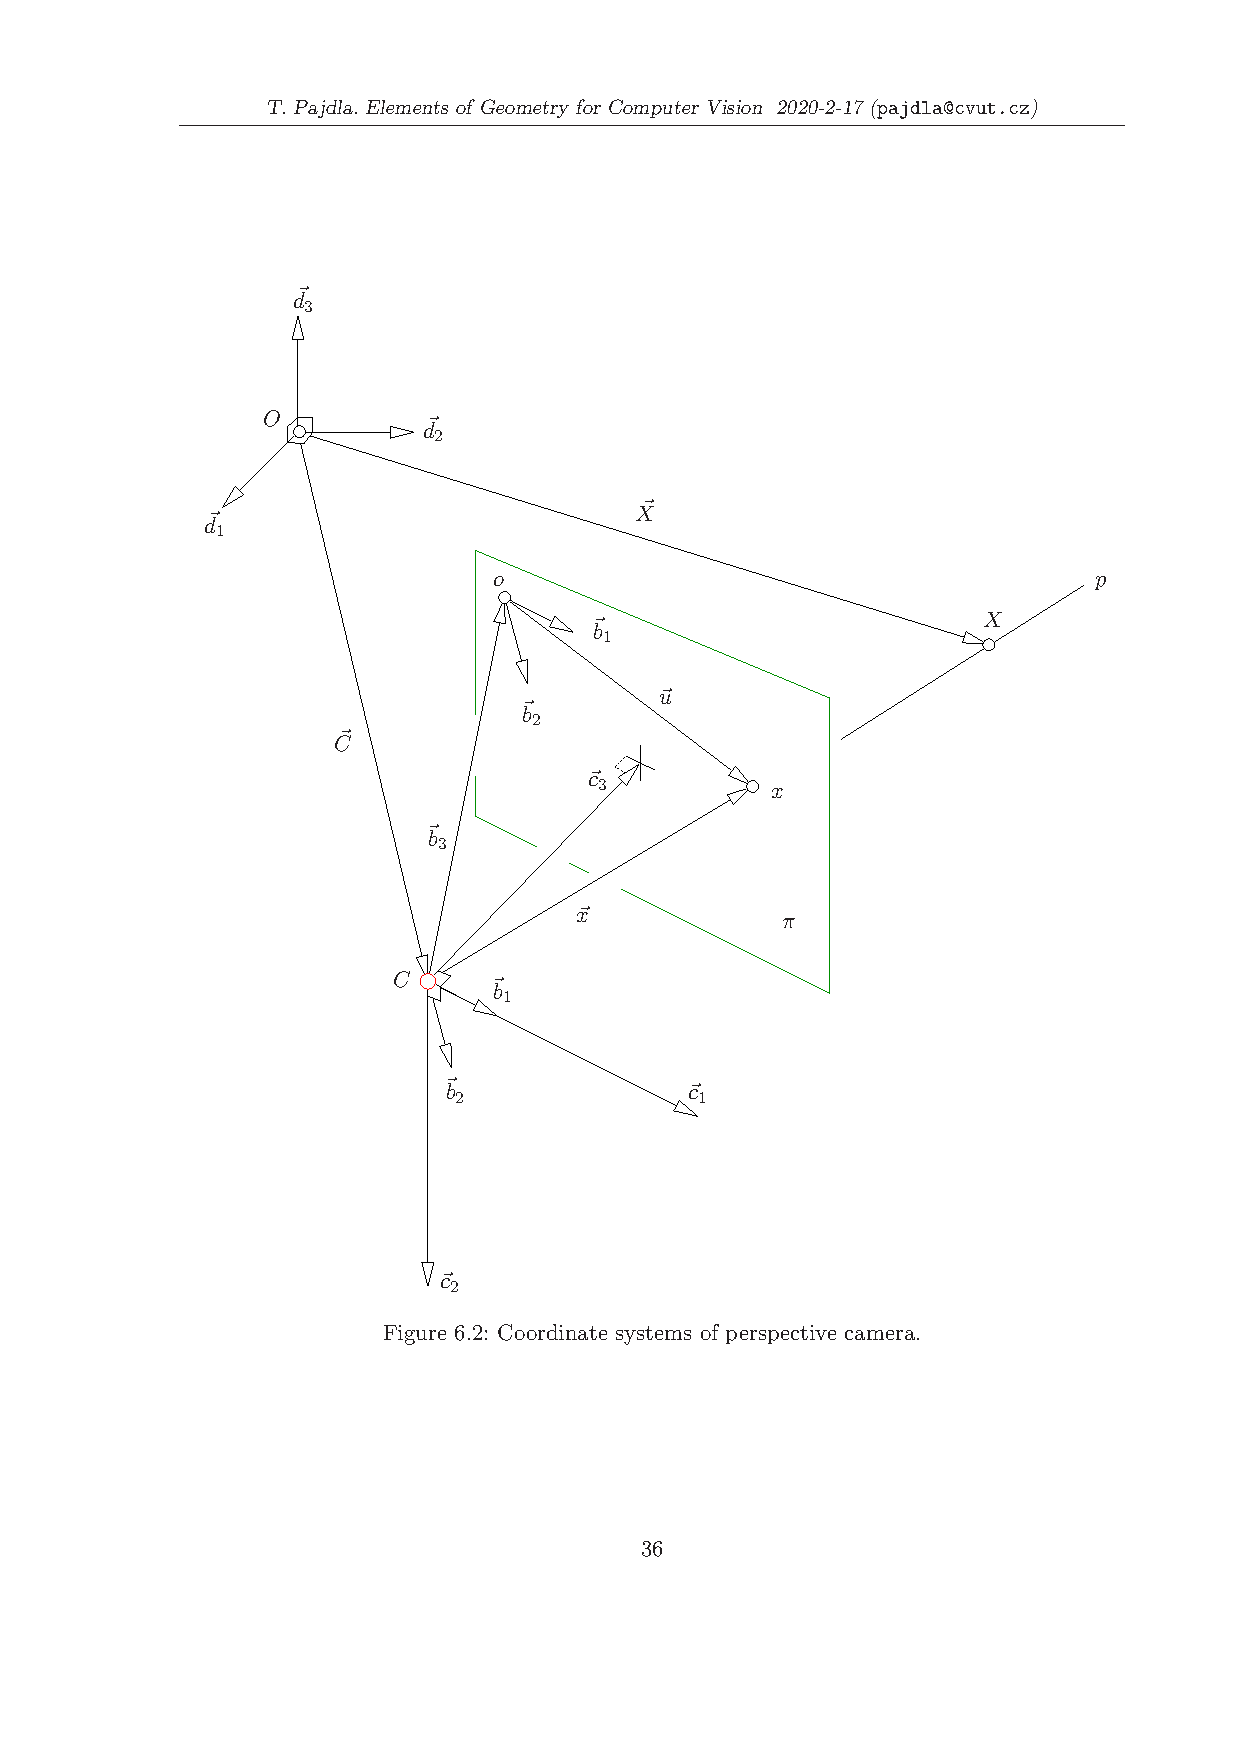
\includegraphics[width=1.0\textwidth,viewport=2.93cm 7.54cm 19.49cm 25.3cm,clip]{GVG_page_cameraCS.pdf}
	\caption[Camera coordinate system]{Camera coordinate system $\gamma$ with bases $\vec c_1, \vec c_2, \vec c_3$; and with origin at $\vec C$ with respect to some World coordinate system $\gamma$. Camera points the $\vec c_3$ direction, having $\vec c_1$ on its right. $\vec b_3$ defines the origin of image coordinate system (pixel at 0,0). Vectors $\vec b_1, \vec b_2$ are considered to be orthogonal, as we are dealing with a rectangular sensor in this thesis. Point $X$ with 3D coordinates $\vec X$ projects onto the image plane to a point $x$ with image coordinates $\vec u$. The two points form a 2D-3D correspondence. Figure is from \cite{GVG}.}
	\label{fig:cameraCoordinateSystem}
\end{figure}

\paragraph{Calibration matrix}
A camera calibration matrix K is a linear transformation that converts points in camera coordinate system $\gamma$ into points in image coordinate system $\beta$. It is defined by five parameters \cite{GVG}:

\begin{equation}
	\text{K} = \begin{bmatrix}
		k_{11} & k_{12} & k_{13} \\
		0 & k_{22} & k_{23} \\
		0 & 0 & 1
		\end{bmatrix}.
\end{equation}

They represent focal length, sensor dimensions, origin of the image coordinate system and more.

Our implementation, however, only requires a subset of those parameters. Thus the calibration matrix K can be constructed as:

\begin{equation}
	\text{K} = \begin{bmatrix}
		f & 0 & w/2 \\
		0 & f & h/2 \\
		0 & 0 & 1
		\end{bmatrix},
\end{equation}

where $w$ and $h$ are width and height of the camera sensor in pixels. Focal length $f$ is also in pixel units.

\section{Multi-camera pose estimation}

Throughout this work, we often operate on query images that were taken in a sequence. Imagine a person walking around a room and taking a picture every once in a while. Considering the sequential nature of the queries can help us improve the localization performance. To achieve this, we need to be able to estimate poses of multiple cameras in the sequence. In general, these cameras are referred to as a rig of cameras. The generalized pose-and-scale problem (GP4Ps/gsP4P), defined in \cite{Kukelova2016CVPR} describes such a problem in general and provides an efficient solution. A particular implementation of the solver is provided as an open source software, named \code{MultiCameraPose}. The project is a result of a recent work \cite{MultiCameraPosePaper}. For my use-case, I modified the implementation slightly and it is available at \cite{MultiCameraPose}. The implementation is very fast, computing the pose estimates of a rig with 5 cameras in about 60 milliseconds. A concrete usage of the \code{MultiCameraPose} program and the changes I have made are described in the Implementation chapter \ref{chapter:implementation}.

\section{Procrustes analysis}
\label{section:procrustes}
Consider two $k$-tuples containing points in $n$-dimensional space:

\begin{equation}
	X = (\vec x_1,\ \vec x_2,\ ...,\ \vec x_k),
	Y = (\vec y_1,\ \vec y_2,\ ...,\ \vec y_k).
\end{equation}

We wish to find an (approximate) linear transformation for the corresponding pairs of points:

\begin{equation}
	\vec x_i \approx \text{T} \cdot \vec y_i, \quad \forall i \in [1,k].
\end{equation}

This is especially meaningful if:

\begin{enumerate}
	\item Points in $X$ are all with respect a common coordinate system, call it $\alpha$.
	\item Points in $Y$ are all with respect a common coordinate system, call it $\beta$.
	\item The points $\vec x_i$ and $\vec y_i$ represent (with possible noise) a common point in $\alpha$.
\end{enumerate}

Procrustes minimizes the sum of squared errors of points:

\begin{equation}
	\argmin_{\text{T}} \> \sum_{i=1}^k{(\vec x_i - \text{T} \cdot \vec y_i)^2}.
\end{equation}

We will be using an implementation in MATLAB called \code{procrustes}; it is available as part of the Statistics and Machine Learning Toolbox \cite{MatlabStats}.

\section{Devices used}
\paragraph{Matterport}
Matterport is a device capable of creating a 3D map of indoor environments. Compared to the Faro 3D scanner used in InLoc dataset \cite{taira2018inloc}, Matterport is a cheaper alternative. Matterport operating time is also lower, and the resulting point cloud is of lower quality \cite{wijmans17rgbd}.

\paragraph{Vicon}
Vicon is a stationary system capable of tracking an object's pose with high accuracy \cite{Vicon}. The tracked object, Marker, contains spheres which have a reflexive surface. Vicon is used for reference pose determination in the newly created dataset within this work.

\paragraph{HoloLens}
HoloLens is a mixed reality device. Mixed reality (MR) is the blending of virtual and real environment, such that the user of MR can interact with both of these environments; see \cite{VR_AR_MR_taxonomy} for a difference between augmented reality, virtual reality and mixed reality. HoloLens is a head-worn device capable of mapping the real environment and localizing itself within it \cite{HoloLensEvaluation}. In this thesis, we are making use of the 1st generation HoloLens \cite{HoloLens1stGen}, referred to as \emph{HoloLens} for simplicity.

HoloLens contains the following sensors \cite{HoloLensEvaluation} \cite{HoloLens1stGen}:

\begin{itemize}
	\item main RGB camera,
	\item 4 environment-understanding grayscale cameras,
	\item a depth sensor,
	\item 4 microphones,
	\item other sensors.
\end{itemize}

The environment mapping and localization are done directly on the device in real-time in a SLAM\footnote{See \cite{SLAM1}, \cite{SLAM2}, \cite{SLAM3}.} -like manner \cite{HoloLensEvaluation}. In an experiment conducted in \cite{HoloLensEvaluation}, the poses estimated by HoloLens had the following mean accuracy with respect to the ground truth poses:

\begin{itemize}
	\item 1.6 $\pm$ 0.2 cm translation error,
	\item 2.2 $\pm$ $0.3\degree$ orientation error.
\end{itemize}

\section{InLoc improvement}
The paper called \emph{Is This the Right Place? Geometric-Semantic Pose Verification for Indoor Visual Localization} \cite{IsThisTheRightPlace} suggests an improvement to the original InLoc. It focuses on significantly improving the the pose verification step. Neither the source code nor the data have been published as of August 9, 2020; and there exists no other open-source implementation to my knowledge. Implementing the methods in this paper would be very time consuming; thus, the results of this paper are not used in our work.

\section{Single View Depth Estimation}
The authors of \cite{SingleViewDepthEstimation} provide a method for learning a convolutional neural network (CNN). The network's task is to, given an input RGB image, estimate the depth of each pixel. The impact of their work is that they managed to do so in unsupervised fashion; eliminating the cost of manually labelling the data \cite{SingleViewDepthEstimation}. The results of that paper could be useful to us, as we could use it to create depth data to improve localization accuracy. However, HoloLens already includes a depth sensor \cite{HoloLensEvaluation}. Although the sensor provides a limited field of view (FoV), it shall be first tested, whether the sensor data are sufficient for our purposes.

\section{Deep Depth Completion}
The paper \cite{DeepDepthCompletion} also provides a solution to the problem of depth estimation from a single RGB image. However, it makes use of the device's depth sensor, builds upon it and improves its accuracy. The problem with many depth cameras is that they often fail to sense depth for shiny, bright, transparent, and distant surfaces \cite{DeepDepthCompletion}. This work, while promising, shall only be considered after we find that the HoloLens depth camera is not sufficient for our purposes.

\section{Marker-based HoloLens localization}
In the paper \cite{HoloLensMarkerBasedLocalization}, authors suggest a method for improving the localization capability of 1st generation HoloLens. They do so by placing markers (2D QR code-like objects) across the environment. The method then allows them to accurately place large virtual models into the environment within a spatial accuracy of few centimeters \cite{HoloLensMarkerBasedLocalization}. The problem of this approach is that it requires the knowledge of the location of the markers with respect to some model coordinate system.

\section{Augmenting Microsoft’s HoloLens with vuforia tracking for neuronavigation}
Paper \cite{HoloLensVuforia} describes a significant improvement of HoloLens accuracy in a medical scenario. It does so by using proprietary Vuforia SDK. The proprietary aspect of it is, however, not ideal for open-source projects.

\section{Magnetic field and Visual Sensors for Indoor Localization}
Paper \cite{MagneticAndVisualIndoorLocalization} shows how to improve localization accuracy by using both visual sensors and a magnetometer. The magnetometer is only present in 2nd generation HoloLens, which we do not have access to. We could use a custom sensor and attach it to the device, however.

\section{Visual Indoor Localization in Known Environments}
The article \cite{VisualIndoorLocalizationInKnownEnvironments} suggests a different approach from InLoc to tackle the indoor localization problem. Instead of constructing a 3D model of the environment in the first stage, visual features are detected in a video sequence and SURF features \cite{SURF} are extracted. According to the article: ``the sequence must cover all the areas in which localization will be needed. ... each
frame is manually labeled with positional information with a
time-consuming procedure''. During the localization, query video frames are matched to frames in the reference video sequence.

This article may be worth considering when we do not have access to a dedicated 3D-environment scanning device.

\section{Multi-sensor-based Indoor Localization System}
The authors of \cite{MutliSensorLocalization} propose a method for robust indoor localization integrating multiple sensors and a visual localization from a single RGB camera. Promising results are shown, but I was unable to find a reference implementation. Creating my own based on the paper would be very time consuming.

\chapter{Dataset}
\label{chapter:dataset}
The original InLoc implementation is using the InLoc dataset \cite{taira2018inloc}, which is based on data taken at the Washington University in St. Louis (WUSTL dataset \cite{wijmans17rgbd}). The InLocCIIRC dataset aims to keep the same structure as the InLoc dataset. The new dataset was created at the Czech Institute of Informatics, Robotics and Cybernetics (CIIRC).

The dataset is a result of scanning two rooms at CIIRC: the B-670 lecture hall and a room B-315. For scanning the environments, a Matterport 3D scanner is used. Let's call the environments \emph{spaces}. Compared to the Faro 3D scanner used in InLoc dataset \cite{taira2018inloc}, Matterport is a cheaper alternative. Matterport operating time is also lower, and the resulting point cloud is of lower quality \cite{wijmans17rgbd}. Matterport creates a point cloud and a mesh model of each space. This is made possible by scanning the area at various locations. Let's call each such scan a \emph{sweep}, to match the Matterport API terminology. To construct the models, RGBD panoramas are taken around the rooms. In B-670, I have taken 31 such panoramas. In B-315, I have taken 27 panoramas. Overall, there are 58 RGBD panoramas taken by Matterport 3D scanner. The scanner was mounted on a tripod at height of approximately 1.52cm and I tried to avoid walls and objects in 60cm radius.

When creating an RGBD panorama, the Matterport scanner has to revolve around yaw axis in order to capture the scene in $360\degree$. For each RGBD panorama, we are given the pose of the Matterport scanner at the moment right before the rotation started. These poses are provided by Matterport, so we don't have to go through the hurdles of estimating them ourselves as in \cite{wijmans17rgbd}.

Another outcome of the sweeps are RGB panoramas. Matterport does not support automatic gathering of these panoramas, so they have to be downloaded manually for every sweep. Another problem is that these downloaded RGB panoramas are not pointing the same direction as is the initial orientation of the Matterport camera. Therefore, I have created a tool to semi-automatically find the proper orientations. This is done by

\begin{enumerate}
	\item projecting the point cloud model according to the sweep pose,
	\item sampling the RGB panoramas around the yaw axis and picking such a sample that best matches the projection. The matching is done by picking such a sample for which the amount of edges in a differential edge image is minimal.
\end{enumerate}

This approach works well, however it may still fail in an exceptional case. Then, a user is encouraged to try the 2nd lowest amount of edges, 3rd least amount and so on. Alternatively, one may try to increase the point size of projected the model. As a last resort, one can manually find the RGB panorama sample by observing all perspective projections of that panorama, generated via a provided script.

Once we have the RGB panoramas which are pointing the same direction as the RGBD panoramas, we can move onto the next stage. Here we construct cutouts, which are perspective projections of the RGB panoramas at a specific orientation. As in InLoc, I am sampling around the yaw axis per $30\degree$, under the pitch direction of $\{-30, 0, 30\}$ degrees. The cutouts also contain information about the depth (not provided by Matterport).

The dataset contains sets of query images (queries). The first set, called s10e, was taken by a smartphone camera --- via Samsung Galaxy S10e's wide angle rear facing lens (i.e. the main lens). I have taken 40 query images in a restricted area of room B-315. This room was chosen to be in the dataset, because it contains a pose estimation system called Vicon. The other two sets of queries were obtained using 1st generation HoloLens; and were also taken in that restricted area. The sets are named HoloLens1 and HoloLens2 --- the suffix number indicates the sequence number. The major difference between s10e and HoloLens query datasets is that the queries from HoloLens form a sequence of images, as the user walked around the room. The sequential nature of those query datasets shall be leveraged, and data from multiple cameras may be used for a higher-precision pose estimation of a current frame.

All of the query images were taken in this specific area of room B-315, so that their reference pose is known. No queries were taken in room B-670, as it would be time consuming to estimate the reference poses manually (or creating a program that does this). Hence, its only purpose is to serve as a confuser.

The queries in the s10e set have a pixel resolution $4032 \times 3024$. InLoc implementation requires the knowledge of focal length of the camera that was used when taking the query images. I found conflicting information about the S10e's field of view (FoV) online, and the focal length didn't add up. I ended up computing the focal length manually with the help of a tripod and a ruler. The focal length turned out to be 3172 pixels. The IDs of query images are sorted in a non-decreasing difficulty, e.g. queries with IDs 1 to 10 were taken such that the camera's direction vector is roughly parallel with the floor. Queries with higher IDs have the camera rotated on a tripod under any direction.

The HoloLens queries have a pixel resolution of $1344 \times 756$ pixels and according to the official documentation, the horizontal FoV is $67\degree$. Because the results were not very precise at some point of development, I began to question whether the documented FoV of $67\degree$ is indeed true. Looking at the data generated while capturing the sequences, HoloLens provides a \code{cameraProjectionTransform} matrix. According to an article \cite{HoloLensFoV}, the effective hFoV can be computed as

\begin{equation}
	\text{\code{hFoV}} = 2 \cdot \arctan \left(\frac{1}{\text{\code{cameraProjectionTransform.m11}}}\right),
\end{equation}

which gives the value of 65.83 degrees. This is the more accurate result, as a reprojection error was lower with this redefined constant.

The sweeps, used to construct the point cloud model, were taken on Thursday/Friday midnight. The s10e query images were taken on a Monday morning 3 days later. Note that there was a weekend between the two time frames, meaning the scene didn't change a lot during that time. The reason the query images were taken later was to test what happens when items such as chair, lighting and people move around or change.

The two HoloLens sequences were captured about three weeks later. This means the environment was more challenging to work with, because it has changed from the state in which it was scanned by Matterport.

Alignments define the pose of individual sweeps within the space they are in. Because the poses are given to us from Matterport, we do not need to perform the generalized iterative closest point (GICP) step, as in InLoc. Because Matterport gives us an entire model (point cloud and mesh) of each scanned space, we do not need to consider alignments at all. They were useful in InLoc, where there were individual point clouds for sweeps and thus the 3D coordinates of the points projecting onto cutouts were wrt the sweep coordinate system.

In InLoc, there are point cloud models for every sweep. On the contrary, in InLocCIIRC we have a model for each space.

The InLoc implementation requires the knowledge of scores between every pair of a query image and a cutout image. An individual score describes similarity between the two images. When the software is run, InLoc chooses, for each query, top N cutouts with the highest scores. The other cutouts will not be considered. It is thus quite important that these scores are relevant. NetVLAD \cite{Arandjelovic16} descriptors are computed for both cutouts and query images. The features are the output of the L2 normalization layer. A score between a query image and a cutout is computed using a dot product between the two feature vectors. Note that the similarity scores of cutouts for a query do not represent a probability distribution, and thus don't need to sum up to one. The code for doing so was not provided in InLoc, so I came up with an implementation that reuses existing InLoc MATLAB components. The resulting scores seem to be meaningful, but a reference implementation would have been better.

\section{Reference poses}
\label{section:reference-poses}
We need to know the reference pose of each query, in order to evaluate how accurate the pose estimation algorithms are. The pose of the cameras used to take the query pictures in query sets was also being tracked by a pose estimation system -- Vicon. Figure \ref{fig:s10e-marker} shows the s10e camera (thus also its coordinate system) and a coordinate system that is being tracked by Vicon. Let the latter coordinate system be called Marker. 

\begin{figure}
	\centering
	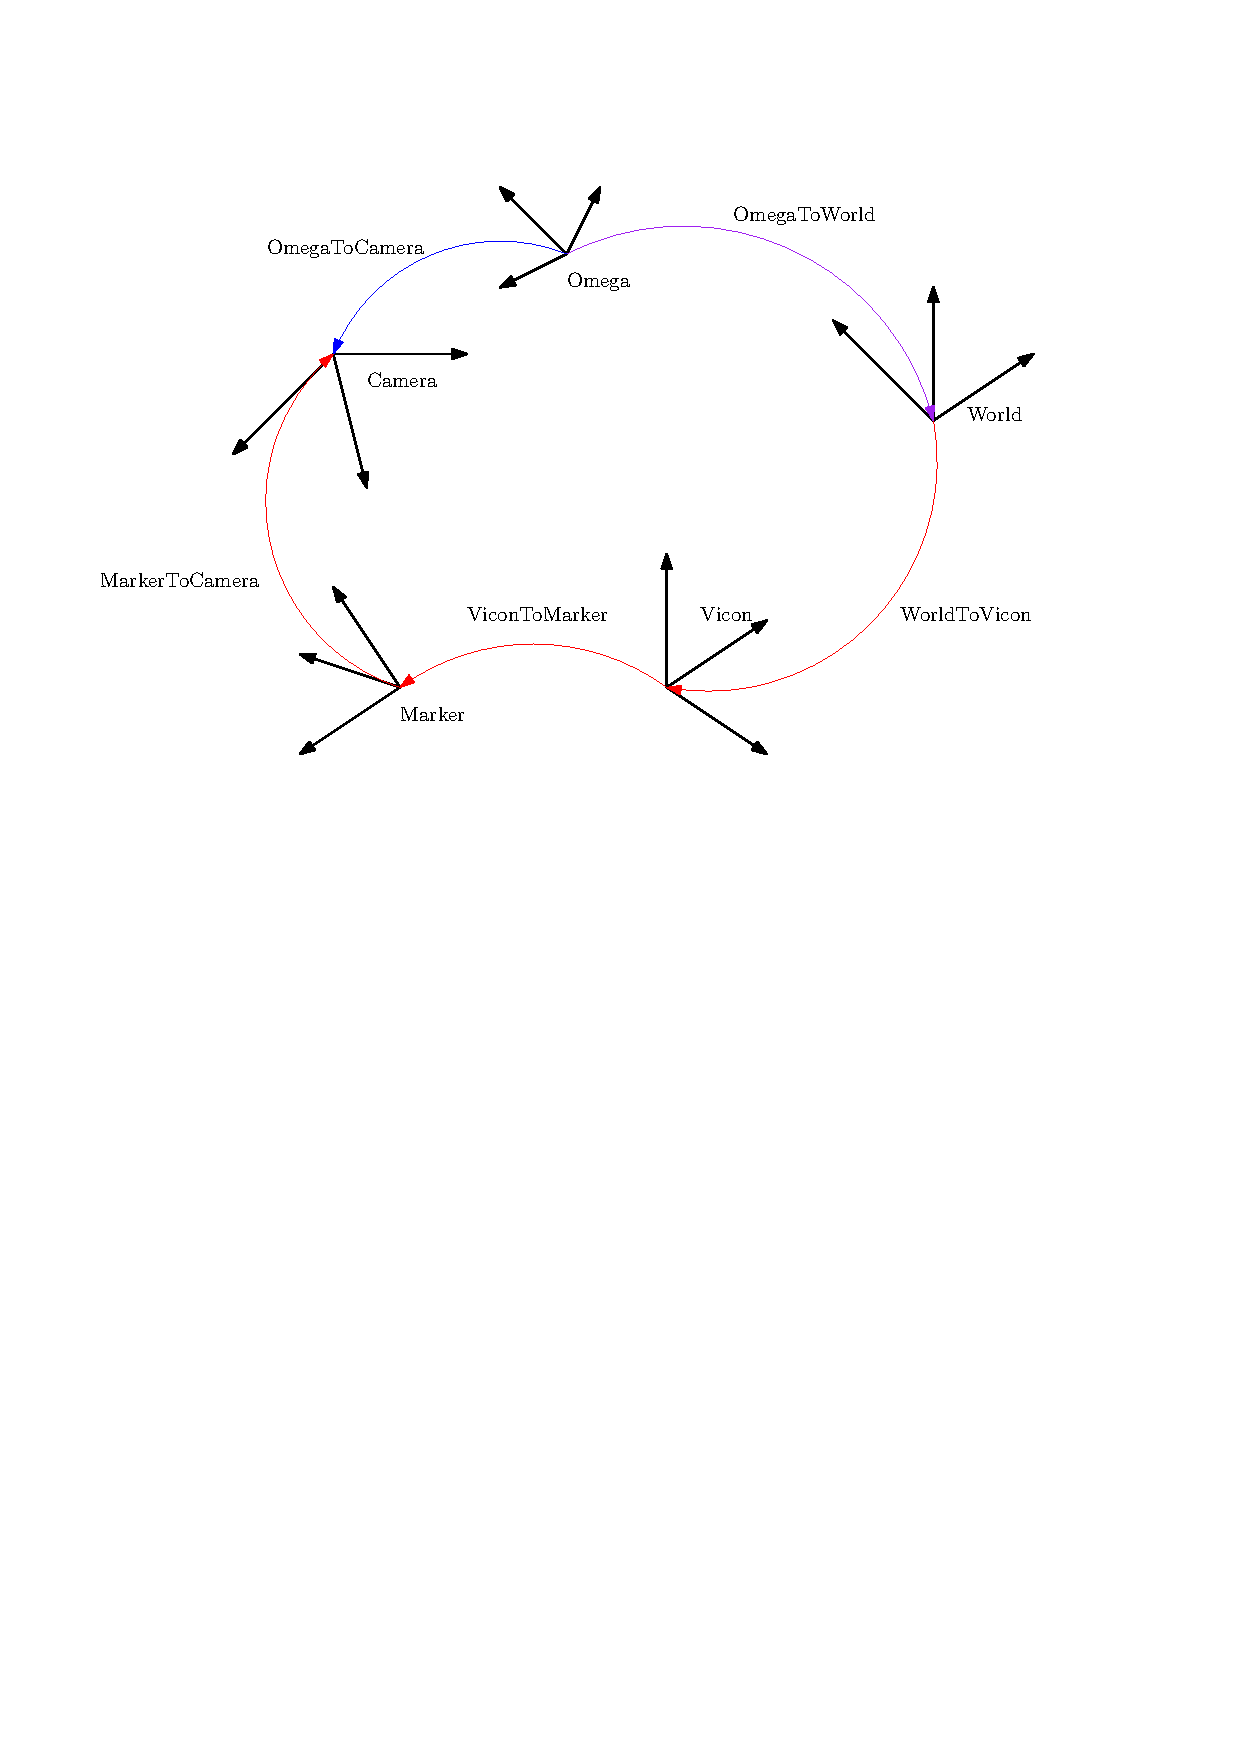
\includegraphics[width=\textwidth]{coordinateSystems.pdf}
	\caption[Coordinate systems in use]{Visualization of the coordinate systems we are dealing with. Omega is the initial unknown HoloLens CS (see section \ref{section:cameraCS} for a an example of a coordinate system). Notice that Omega has a scaling independent of the World CS scaling. Linear transformations are shown by the arrows. There are in fact two slightly different Camera coordinate systems -- one that is estimated from HoloLens and another one (reference pose) that is estimated using Vicon. OmegaToCamera is known for most\protect\footnotemark of the HoloLens queries, because the data comes from HoloLens. ViconToMarker is provided from Vicon tracking. WorldToVicon has been manually determined. MarkerToCamera has been approximated by an algorithm described in the Reference poses section \ref{section:reference-poses}.}
	\label{fig:coordinate-systems}
\end{figure}
\footnotetext{For exceptions caused by delays take a look at table \ref{tab:HL-pose-delays}.}

\begin{figure}
	\begin{subfigure}{0.45\textwidth}
		\includegraphics[width=\textwidth]{s10e_marker}
		\caption{s10e query set.}
		\label{fig:s10e-marker}
	\end{subfigure}
	\hspace*{\fill}	% maximize separation between the subfigures
	\begin{subfigure}{0.45\textwidth}
		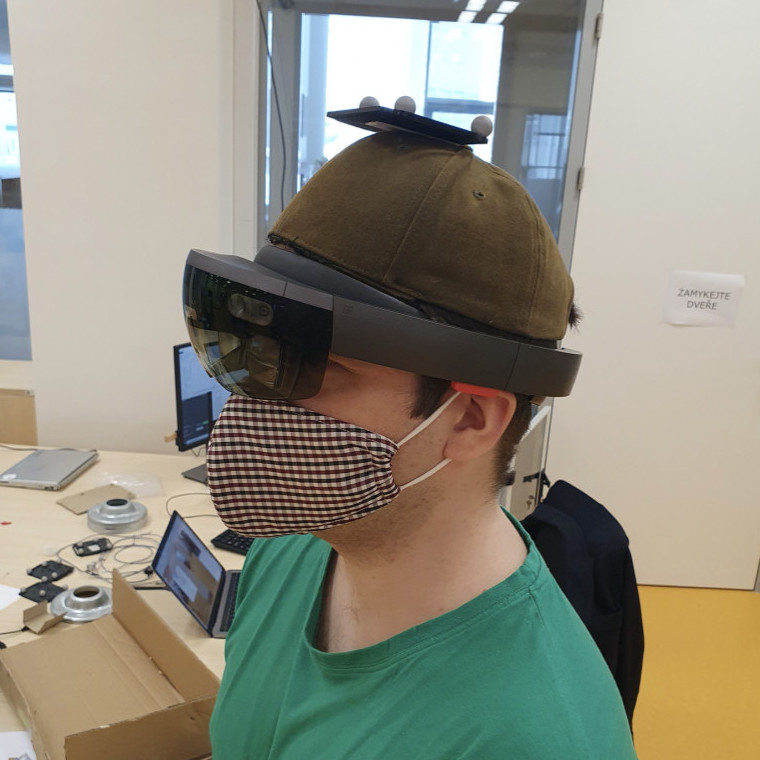
\includegraphics[width=\textwidth]{HL1_marker}
		\caption{HoloLens2 sequence.}
		\label{fig:holoLens-marker}
	\end{subfigure}
	\caption[Camera and Marker]{The camera and marker (the object tracked by Vicon). Marker coordinate system is visualized in subfigure \ref{fig:s10e-marker} by the xyz arrows.}
	\label{fig:camera-markers}
\end{figure}

Let's now focus on a more difficult scenario, which is the reference pose determination of the HoloLens queries. There are three reasons why the reference poses cannot be simply taken from the Vicon tracking:

\begin{enumerate}
	\item camera pose and Marker are widely different,
	\item the Vicon coordinate system differs from the World\footnote{The World coordinate system is a coordinate system of the point cloud and mesh models provided by Matterport.} coordinate system,
	\item Vicon started tracking before HoloLens was run, as visualized in figure \ref{fig:HL_and_vicon_time}.
\end{enumerate}

\begin{figure}
	\centering
 	\includegraphics[width=1.0\textwidth]{HL_and_vicon_time}
 	\caption[HoloLens and Vicon timelines]{Visualization of the HoloLens and Vicon timelines. The synchronization constant must be found. Note that the sampling frequencies are vastly different. However, given a query image from HoloLens taken at some point in time (HoloLens sampling frequency), we find the corresponding reference pose that has the nearest timestamp (after taking the synchronization constant into account; Vicon sampling frequency).}
 	\label{fig:HL_and_vicon_time}
\end{figure} 

Luckily, the second issue turned out to be easily mitigated. I have been told where the origin of the Vicon coordinate system is. And by experimentation, the rotation matrix that converts Vicon bases to World bases was found. Because the Vicon bases and World bases are aligned to the room (i.e. a basic vector is parallel with the floor or the walls), the rotation matrix can be represented by a simple rotation.

The transformation from Marker to camera is considered to be a constant (for all queries in a query set), because the tracking device is securely attached to the camera. One could manually estimate that transformation and visually evaluate how close the model projection is to the original query image. However, this approach is prone to errors. Instead, a quantitative approach was employed, which I describe next.

For a particular query set, we need to manually set up the reference poses for a small number of queries. I used 6 of them in HoloLens1. Let these queries be called \emph{interesting} queries. For such a query, we manually find nine 2D-3D correspondences. The 2D correspondences are carefully chosen, such that they actually represent the same 3D point -- because the 3D points were captured up to three weeks earlier than the query images and the environment has changed. For each query with the correspondences, we compute its initial reference pose using P3P. The pose returned by P3P may not be completely accurate, however.

Given reference poses for 6 queries and corresponding poses from Vicon, we can almost compute individual Marker to camera transformations. The last piece missing is a synchronization constant, to match the correct Vicon pose taken at Vicon time with a particular query taken at HoloLens time. I created a script, \code{findOptimalParamsForInterestingQueries.m}, which computes the Marker to camera transformations and evaluates the reference poses quality both quantitatively (reprojection error) and visually (manually investigated by the user). Currently, user must guess a synchronization constant. Finding a reasonable synchronization constant does not take long. Alternatively, one could implement a brute-force search, where various synchronization constants are guessed and the one with lowest quantitative error is chosen. In my case this was not necessary. At the end of the script, a generic transformation is suggested, which is an average of the individual transformations. The quality of the generic transformation is again evaluated on all the 6 queries. This generic transformation and the synchronization constant are used as a baseline and are further optimized, described next.

A brute-force search is employed to find an improved version of the baseline transformation and synchronization constant in nearby space. First, an improved synchronization constant is estimated, by simply evaluating the interesting queries on the same transformation but for different synchronization constants, that are close to the baseline constant. Then, different transformations are being tried. An Marker to camera transformation is described by a 3D translation vector and a 3x3 rotation matrix. Note that this rotation matrix can be represented by three parameters (yaw, roll and pitch). Thus, the code iterates over predefined values of the 6 parameters, such that every combination is tried. For each combination, the reprojection error is computed and stored for later. The parameters are continuous, but I try a sequence of values nearby the baseline value, with a constant offset. When it comes to the translation parameters, I have had good experience with trying 17 values, where the middle value is the baseline. The offset was 0.023 Matterport meters. Each orientation parameter was evaluated on 11 values with even offsets, where the middle value was the baseline. The offset was $0.5\degree$. The brute-force search is very time consuming, taking about 20 hours on a machine capable of processing 45 threads at once. Optionally, one can iterate over 5 synchronization constant values, for even more optimal parameters to be found. Of course, by doing that, the search will take asymptotically 5 times as much time and memory resources.

Table \ref{tab:HL1-ref-poses-errors} shows quantitative evaluation of the quality of reference poses, after the brute-force optimization. Table \ref{tab:HL1-ref-non-optimized-poses-errors} shows the same statistics for parameters prior to the optimization (baseline transformation). The improvement is not significant: 1 cm lower translation error and $0.14\degree$ lower orientation error. Figure \ref{fig:interesting-reprojection-s10e-query-2} shows an example of the 9 manually defined correspondences and their reprojection errors.

\begin{table}
	\begin{subtable}{.9\linewidth}\centering
		{
		\footnotesize
		\begin{tabular}{|r|c|c|c|}
			\hline
			Query ID & Average projection error [px] & Sum of projection errors [px] \\
			\hline
			1 & 3.47 & 31.24 \\
			94 & 9.80 & 88.19 \\
			237 & 10.06 & 90.52 \\
			281 & 3.83 & 34.48 \\
			155 & 5.07 & 45.63 \\
			198 & 3.23 & 29.10 \\
			\hline
			\hline
			Sum & N/A & 319.16 \\
			\hline
		\end{tabular}
		}
		\caption{Reprojection error.}
		\label{tab:interesting-reprojection-s10e}
	\quad
	\end{subtable}
	\begin{subtable}{.9\linewidth}\centering
		{
		\footnotesize
		\begin{tabular}{|r||c|c|}
			\hline
			& Mean errors & Standard deviation of errors \\
			\hline
			Translation [m] & 0.15 & 0.08 \\
			Orientation [m] & 2.09 & 1.69 \\
			\hline
		\end{tabular}
		}
		\caption{\HLvsRefPosesErrorsCaption{}}
		\label{tab:HL1-ref-vs-HL-errors}	
	\end{subtable}
	\caption[Evaluatio of optimized HoloLens1 reference poses]{Quantitative evaluation of reference poses quality. HoloLens1 sequence shown. Parameters describing the Marker to camera transformation were \textbf{optimized} using brute-force search.}
	\label{tab:HL1-ref-poses-errors}
\end{table}

\begin{figure}
	\centering
 	\includegraphics[width=0.80\textwidth]{HL1-query2-reprojection}
 	\caption[Reprojection error on optimized s10e parameters]{Query 94 of HoloLens1 and its reprojections errors. The optimized transformation params were used. The same image on non-optimized parameters is not shown, because the average improvement of reprojection error of a the correspondences is about 2 pixels. Therefore a naked eye can barely tell which image has lower reprojection error. Green points: optimal location of 2D correspondences. Red dots: location of the 3D correspondences (projected onto 2D image plane), under the generic parameters (that aim to work across all queries in the sequence).}
 	\label{fig:interesting-reprojection-s10e-query-2}
\end{figure} 

\begin{table}
	\begin{subtable}{.9\linewidth}\centering
		{
		\footnotesize
		\begin{tabular}{|r|c|c|c|}
			\hline
			Query ID & Average projection error [px] & Sum of projection errors [px] \\
			\hline
			1 & 3.38 & 30.42 \\
			94 & 11.96 & 107.66 \\
			237 & 9.22 & 82.98 \\
			281 & 3.62 & 32.57 \\
			155 & 5.99 & 53.91 \\
			198 & 3.08 & 27.68 \\
			\hline
			\hline
			Sum & N/A & 335.22 \\
			\hline
		\end{tabular}
		}
		\caption{Reprojection error.}
		\label{tab:interesting-reprojection-non-optimized-s10e}
	\quad
	\end{subtable}
	\begin{subtable}{.9\linewidth}\centering
		{
		\footnotesize
		\begin{tabular}{|r||c|c|}
			\hline
			& Mean errors & Standard deviation of errors \\
			\hline
			Translation [m] & 0.16 & 0.08 \\
			Orientation [m] & 2.23 & 1.62 \\
			\hline
		\end{tabular}
		}
		\caption{\HLvsRefPosesErrorsCaption{}}
		\label{tab:HL1-ref-non-optimized-vs-HL-errors}
	\end{subtable}
	\caption[Evaluation of non-optimized HoloLens1 reference poses]{Quantitative evaluation of reference poses quality. HoloLens1 sequence shown. Tables show performance on the parameters, describing the Marker to camera transformation, \textbf{prior} using brute-force search optimization.}
	\label{tab:HL1-ref-non-optimized-poses-errors}
\end{table}

\phantomsection
\label{paragraph:gt-vs-ref-poses}
The resulting reference poses are not perfectly matching ground truth poses, which can be seen when projecting the reference poses and comparing the results with the query images. I have created the following procedure in order to estimate the mean translation and orientation error (reference vs ground truth poses). Although we do not know the true ground truth poses, one can use the poses from HoloLens. According to \cite{HoloLensEvaluation}, the poses estimated by HoloLens have the following mean accuracy with respect to the ground truth poses:

\begin{itemize}
	\item 1.6 $\pm$ 0.2 cm translation error,
	\item 2.2 $\pm$ $0.3\degree$ orientation error.
\end{itemize}

Notice that namely the the translation error is very low. To estimate the quality of my reference poses wrt ground truth poses, I consider the HoloLens poses as the ground truth poses. However, because the poses from HoloLens are wrt some unknown initial HoloLens coordinate system (Omega), I first need to convert those poses to be wrt World. To achieve this, I use procrustes \cite{procrustes}, which finds a linear transformation from one coordinate system to another (translation, rotation, scale), given corresponding 3D points. In my case, the 3D points are simply the camera centers. Procrustes minimizes the sum of squared errors of points in the same coordinate system. After the conversion, we would have ground truth estimates.

Unfortunately, there was another hidden problem that had to be dealt with, prior the reference vs ground truth pose errors could be computed. The problem is that the poses provided from HoloLens do not correspond to the query they are associated with in the data. It turns out the poses are delayed. To make matters worse, both the translation and orientation that are used to construct the camera pose are delayed by a different amount! To resolve this issue, the pose from HoloLens associated to a query is computed to be based on translation and orientation data, that comes from the future queries. I found that the best results were achieved with the delays in table \ref{tab:HL-pose-delays}.

\begin{table}[ht]
    \centering
    {\footnotesize
	\begin{tabular}{|c|c|}
	\hline
	Type & Number of frames \\[1pt]
	\hline
	Translation delay & 6 \\[1pt]
	Orientation delay & 4 \\[1pt]
	\hline
    \end{tabular}
	\caption[Optimal HoloLens delay parameters]{We are using a program \cite{HoloLensDataAcquisition} for fetching data from HoloLens. It provides a CSV file containing information on the query images it took, when they were taken (timestamp), estimated poses and more. The camera pose estimates are represented by translation and orientation parameters, which are in Omega coordinate system. However, these parameters are wrongly assigned, as they are in fact delayed by a number of frames. The time difference between two consecutive frames is about 333 milliseconds. Optimal delays for HoloLens1 sequence are shown.}
	\label{tab:HL-pose-delays}
    }
\end{table}

A consequence of the data being delayed is that, for some of the queries at end of the sequence, we do not have the poses from HoloLens available. Recall also that some reference poses are blacklisted, because Vicon got lost.

Using these delays and the \code{procrustes} method\footnote{See section \ref{section:procrustes}.}, we can compute the mean reference vs ground truth pose errors, which is:

\begin{itemize}
	\item 15 cm translation error,
	\item $2.09\degree$ orientation error.
\end{itemize}

These errors may be either an upper bound (the data being delayed may still cause trouble) of the real mean errors, but they can also be approximately the true mean errors. As you can see, the translation error is significant. This is concerning, because it will not clear whether our newly developed localization methods are better than the poses provided by HoloLens themselves. Note that in case of s10e queries, the reference poses seem to have a lower error wrt ground truth. However, because we do not know the ground truth and no HoloLens poses are available here, I cannot quantitatively evaluate their quality wrt ground truth (but the reprojection error on the queries that were manually assigned 2D-3D correspondences can be computed).

The query images can be split into two categories --- InMap and OffMap. An InMap query is such a query, for which we have a cutout that has a similar pose. I have defined the pose similarity as:

\begin{itemize}
	\item the translation difference is less than $1.3$ meters,
	\item the angular distance between the reference query and cutout rotation matrices is at most 10 degrees,
\end{itemize}

Where we define the angular distance between two $3 \times 3$ rotation matrices $\text{R}_1$ and $\text{R}_2$, representing two orientations, as:

\begin{equation}
	\label{eq:rotation-distance}
	\left |~\arccos \left(\frac{\Tr (\text{R}_2 * \text{R}_1^{-1})-1}{2} \right)~\right|.
\end{equation}

The set of s10e queries consists of 5 InMap queries and 35 OffMap queries. The set of HoloLens1 queries consists of 111 InMap queries and 239 OffMap queries. The HoloLens2 does not have up to date reference poses. According to an outdated result, it contains 48 InMap and 570 OffMap queries.

The entire dataset, excluding the generated output, occupies about 130 GB of disk space.

The dataset statistics are depicted in table \ref{tab:dataset-statistics}. Notice that the horizontal field of view of database cutout images is widely different from the query horizontal FoVs. When I tried to generate the dataset, such that the cutouts have horizontal FoV of 60 degrees, the resulting pose estimation accuracy became 0\%. I had spent a significant time investigating why this is happening, and came to the conclusion that the problem was in the data. When one creates a cutout of a lower FoV, smaller portion of the $360\degree$ panorama gets rendered. This also means that the visual quality of the image decreases. I believed that the quality of such cutouts is not good enough for the convolutional neural network to generate reasonable feature descriptors. Figure \ref{fig:fov-quality} illustrates this problem. It seemed that there was nothing we can do about it, since the pixel density of each $360\degree$ panorama is determined by Matterport. It is, however, true that one could experiment with other FoV values. Such experiments were not conducted here, as regenerating the dataset and then uploading it to an evaluation server takes a lot of time (one day is not an exception). Why have I used a past tense? The thing is that the experiment, where cutouts with hFoV $60\degree$ are used, took place a while ago. Since then, a couple of bugs in my implementation were fixed. The hFoV $60\degree$ set-up shall be tried again (I did not have the resources to do it).

\begin{table}[t]
    \centering
    {\footnotesize
	\begin{tabular}{|r||c|c|c|c|}
	\hline
	Type & Amount & Without ref. pose & Image size [px] & HFoV [\degree] \\[1pt]
	\hline
    Query - s10e & 40 & 0 & 4,032$\times$3,024 & 64.86 \\[1pt]
    Query - HoloLens1 & 350 & 24 & 1344$\times$756 & 65.83 \\[1pt]
    Query - HoloLens2 & 618 & 299 & 1344$\times$756 & 65.83 \\[1pt]
	Cutout & 2,088 & 0 & 1,600$\times$1,200 & 106.26 \\[3pt]
	\hline
    \end{tabular}
	\caption[Statistics of the InLocCIIRC dataset]{Statistics of the {\bf InLocCIIRC dataset}. Note that some queries are without a reference pose assigned to them. This occurs when Vicon gets lost (returns a non-sense pose for a certain period of time). Such queries are ignored in performance evaluation. Note that the HoloLens2 sequence contains a lot of queries, for which Vicon failed. This may be related to the fact that I moved slighly faster around the room in that sequence, making it harder for Vicon to keep track of the marker. Cutout poses are provided from Matterport and because of their quantity, not all of them were manually verified. For I never discovered a problem with the cutout poses, I consider their poses to be flawless. HFoV stands for the horizontal field of view.}
	\label{tab:dataset-statistics}
    }
\end{table}

\begin{figure*}
    \centering
    {
    \begin{tabular}{c}
    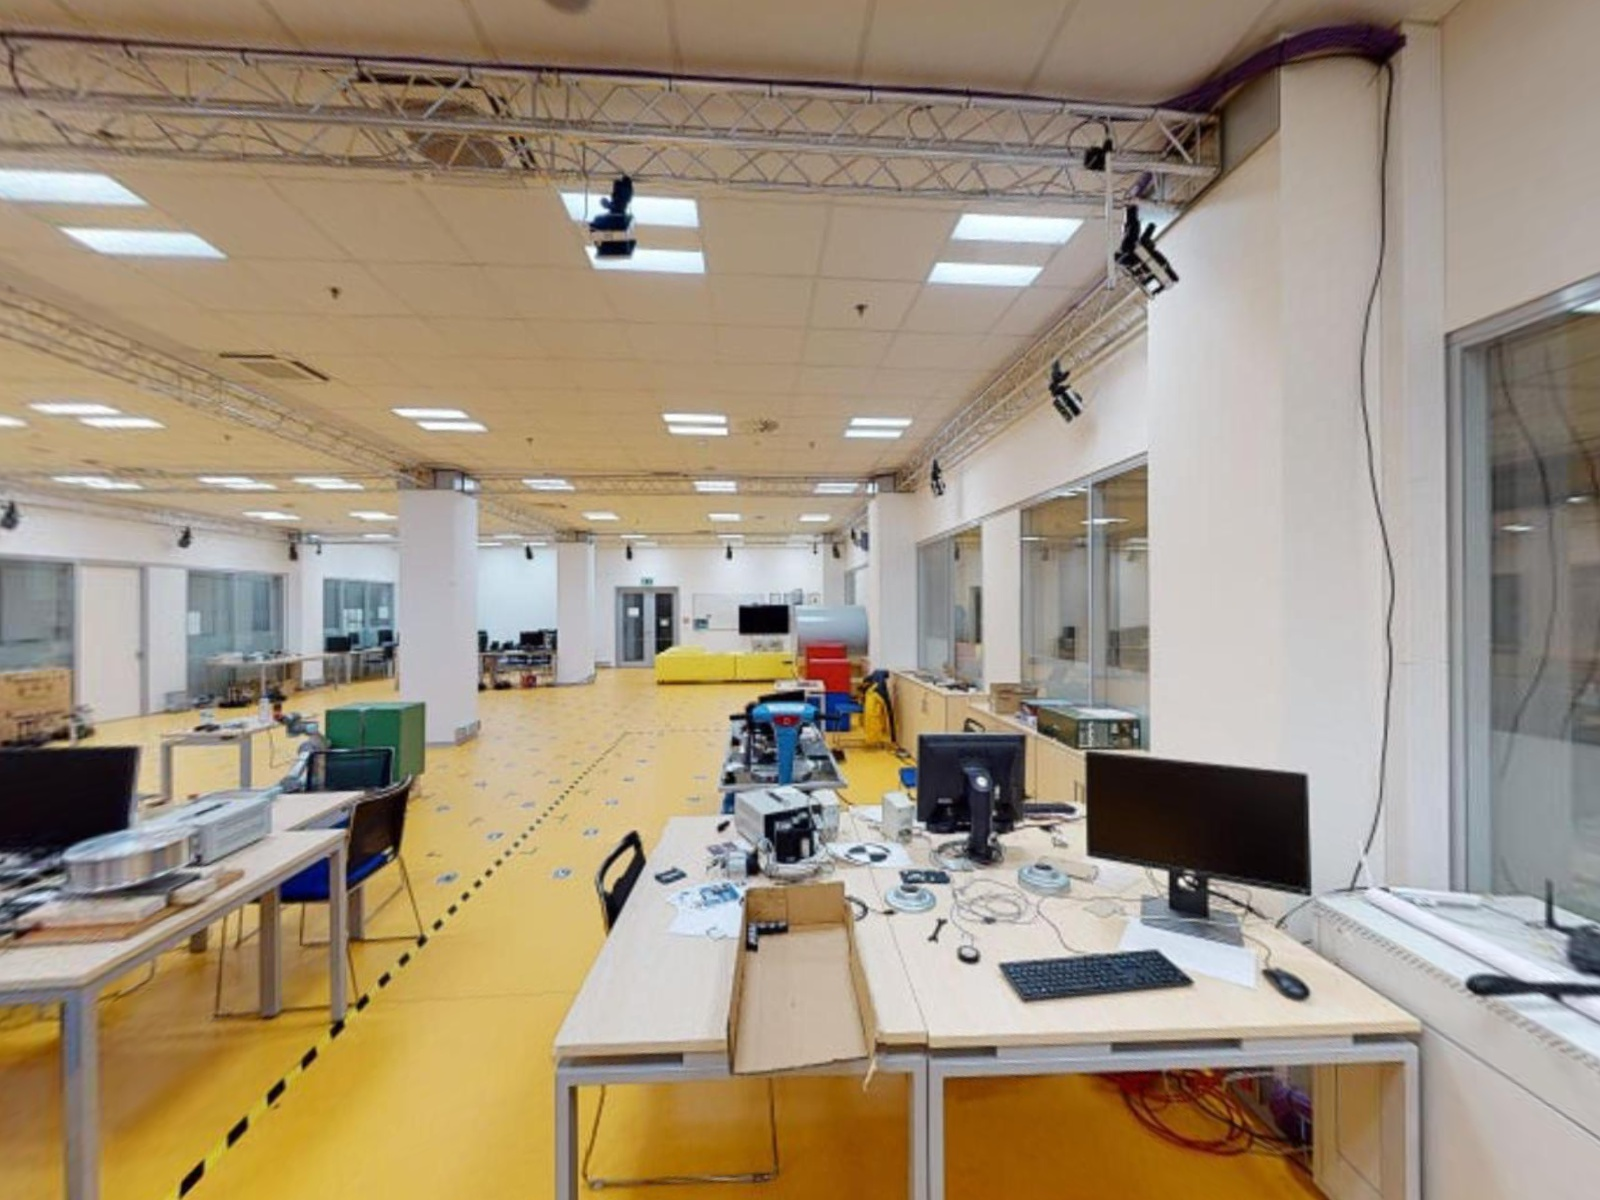
\includegraphics[width=0.8\textwidth]{cutout_19_-90_0_FoV106} \\
    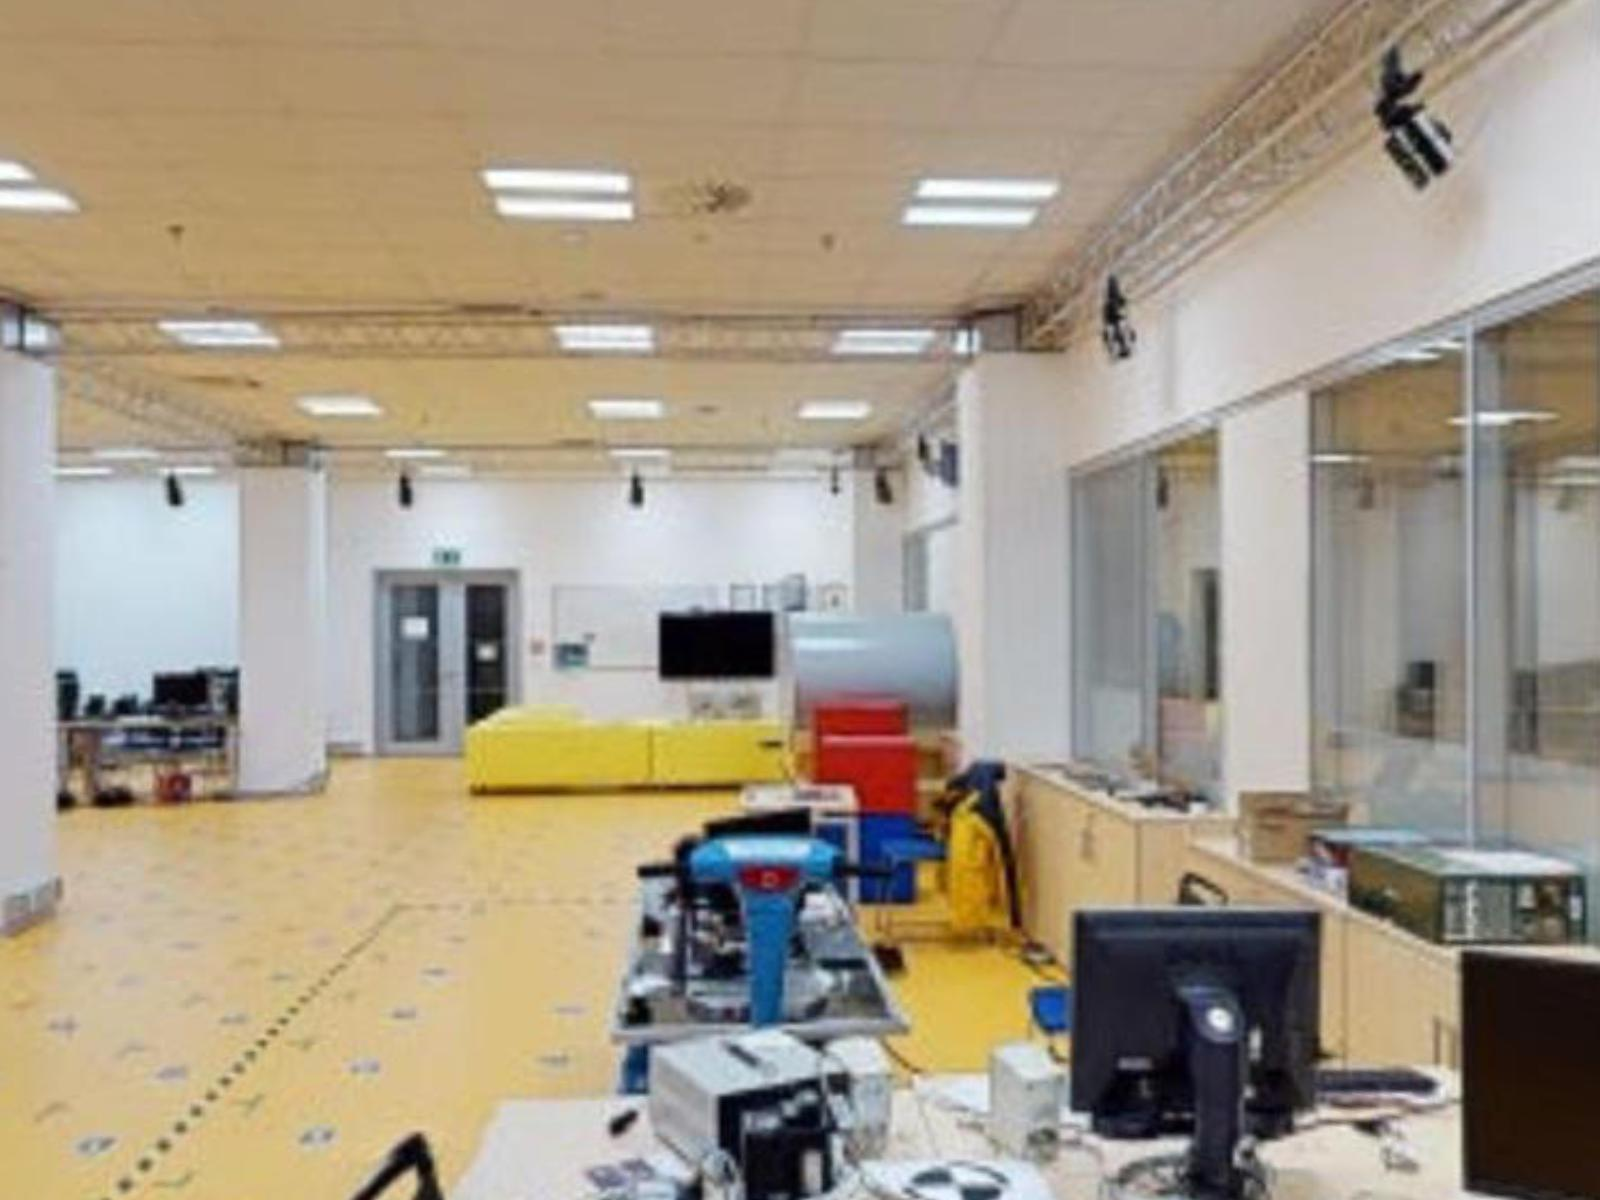
\includegraphics[width=0.8\textwidth]{cutout_19_-90_0_FoV60}
    \end{tabular}
	\caption[FOV quality comparison]{{\bf Visual quality comparision of the same cutout under different FoV.} Top: horizontal FoV: $106.26\degree$. Bottom: horizontal FoV: $60.00\degree$. The image with a lower FoV contains a lot of artifacts and is of lower visual quality.}
	\label{fig:fov-quality}
    }
\end{figure*}

\paragraph{Handling of reflective surfaces}
The scanned rooms contain a couple of types of objects that can confuse the Matterport scanner; luckily, the Matterport Capture iOS app contains tools designed to deal with such problems. After some experimentation, I obtained the highest-quality 3D model with the following settings:

\begin{table}[htb!]
	\centering
	\begin{tabular}{|c|c|}
		\hline
		\bfseries Object type & \bfseries Handling in Matterport \\
		\hline
		\hline
		Outer window & Window \\
		\hline
		Indoor window & Window \\
		\hline
		TV & Default \\
		\hline
		Door with glass elements & Window \\
		\hline
	\end{tabular}
	\caption[Handling of reflective surfaces]{Handling of reflective surfaces in the Matterport Capture app. The options are: Default, Window, Mirror. Best results were obtained using the values in this table.}
	\label{tab:matterport-reflective-surfaces}
\end{table}

\section{Habitat}
We provide an (incomplete) tool for generating synthetic datasets in InLoc dataset-like format. The tool is a modification of the Habitat AI platform \cite{habitat19iccv}. It currently supports creation of sequential query sets in digitalized environments, such as the Matterport3D dataset \cite{Matterport3D} and our InLocCIIRC dataset \todo[podporu pro nas dataset vytvorila martina, tohle bych sem nemel psat!]. The implementation is available at \cite{HabitatFork}. It can be used for creation of large datasets (for evaluation of indoor localization methods) without an expensive 3D scanning equipment. However, evaluating an improved HoloLens tracking accuracy is not very meaningful here, as the data from HoloLens would need to be simulated.

\subsection{Usage}
\begin{enumerate}
	\item Navigate to \code{habitat-api/examples/capture\_sequence.py}.
	\item Choose an environment in the \code{habitat-api/configs/datasets/pointnav/} folder.
	\item Adjust the \code{environmentConfigPath} variable to the selected environment.
	\item Adjust the \code{outputPath} variable.
	\item Run the script.
	\item Navigate around the environment using \code{WASD} and arrow keys.
	\item After each movement, a query image is saved and its pose within that environment stored.
	\item Press \code{F} to exit.
\end{enumerate}

A future work could add support for the creation of the panorama/cutout images.

\chapter{Implementation}
\label{chapter:implementation}

InLoc \cite{taira2018inloc} authors provide a demonstration in MATLAB that operates on the InLoc dataset. I have taken this demonstration and adjusted it, so that it works on the InLocCIIRC dataset instead. I have added an evaluation script, that was missing from the original code. Although the evaluation of InLoc is handled by \url{http://www.visuallocalization.net}, this tool of course doesn't handle the newly created InLocCIIRC dataset yet.

The entire InLocCIIRC implementation should run on a multi-core machine with a GPU. The number of processing CPU threads can be up to 45 at a time. In order to do this, I was running the program on a CMP\footnote{Center for Machine Perception at Czech Technical University in Prague.} server. However, the GPU node prohibited the use of more than 8 CPU threads per user. Therefore the implementation was split into 2 parts: in the first run, the GPU is used; in the latter run, no GPU is required, but a CPU with a lot of cores is used. The need for a GPU comes from the fact that we are using inference of NetVLAD-based neural network, which would take much longer on a CPU. This GPU restriction is present in InLoc implementation as well.

The original InLoc implementation uses point cloud projection in the pose verification step. However, the code for point cloud (PC) projection did not support variable point size. Because the models in my datasets are not dense (compared to those taken with the Faro 3D scanner), the projection can sometimes see through pillars or objects that are close to the camera. This is not desirable, as seeing what is behind the object can result in a different NetVLAD descriptor that is not similar to the query image. At first I have implemented PC projection with a point size parameter, but the problem is that it does not support headless\footnote{Headless rendering is rendering on a computer where the rendering program is not attached to a physical display.} rendering. I ended up using a mesh model projection instead of a point cloud projection in the point verification step. I am using existing software packages to achieve this (\code{pyrender}, \code{trimesh}, \code{open3D}). My \code{projectMesh} method supports headless rendering. Unfortunately, it is very demanding - requires ~14 GB RAM and it also takes time to load the dataset into memory. Of course, one would cache the model in memory and then just call the render functions. However, this would require non-trivial implementation changes, because the implementation is in MATLAB and the \code{projectMesh} routine is in Python.

A major change to the implementation was adding support for sequential queries. Currently the code\footnote{The repository implementing the new pipeline is called \code{InLocCIIRC\_demo}, but the name is in fact not very accurate, because it is not really an implementation of the InLoc paper \cite{taira2018inloc}. However, the pose estimation algorithms are indeed based on InLoc.} supports specifically sequential queries from HoloLens. To estimate poses (wrt World) of sequential queries from HoloLens, poses from HoloLens (wrt Omega) must be provided. The latter poses are computed by HoloLens itself. There are two approaches how the sequential nature of query sets is leveraged. Both approaches depend on a parameter \emph{k}. We want to estimate the camera pose for each query in the query sequence. At each such query, we consider a segment of queries, such that the last query in the segment is the currently processed query. Constant \emph{k} defines how long the segment is.

The first approach is called SequentialPV. It only leverages the other queries (in the segment) in the pose verification step. This approach aims to be more robust than the non-sequential one, by providing more evidence: the projection quality for all queries in the segment is considered and compared to the input query images. How is this done? We have top \topPE{} camera poses (given by P3P in the pose estimation step). These poses are the estimated poses of the current query. Next, we have camera pose estimates for every query in the segment, provided by HoloLens. Those poses are wrt Omega. Therefore, we convert the poses from HoloLens from Omega to World, by aligning the two poses of the last query in the segment. The two poses are:

\begin{itemize}
	\item the camera pose estimate (wrt World) provided from pose estimation step,
	\item the camera pose estimate (wrt Omega) provided from HoloLens.
\end{itemize}

To match the two poses, we just need to compute a linear transformation (rotation, translation). With this transformation, the other poses from HoloLens are converted from Omega to World. With all camera pose estimates being with respect to World coordinate system, we run the pose verification step. The pose verification step returns a score, symbolizing the quality of the input query image and the reconstructed query image. All the scores in the segment are summed up. Note that there are other ways of integrating the scores together: e.g. mean, maximum; I haven't tested them yet. This is done for those top \topPE{} poses from the pose estimation step. At the end, I choose the candidate with highest score to represent the final camera pose estimate. This approach is a basic way to leverage the fact that the queries were taken in a sequence (and captured with HoloLens).

Approach two is called MultiCameraPose. We want to estimate pose of each query in the sequence by taking into account all poses and correspondences in the current segment. The camera pose estimates (wrt Omega) are taken from HoloLens. The 2D-2D correspondences are computed using the geometric verification step and are subsequently converted into 2D-3D correspondences. Given these data, an external program called \code{MultiCameraPose} \cite{MultiCameraPose} processes them and returns the camera pose estimates wrt World. The program contains an implementation of gsP4P \cite{Kukelova2016CVPR}. For details on the \code{MultiCameraPose} program and gsP4P, please see Chapter \ref{chapter:literature-review}. We then store all returned camera rig poses, as the main result of the pose estimation step. In the pose verification step, all the estimated poses within a particular segment are evaluated (score is computed). Again, the candidate segment with the highest cumulative (summed up) score is selected. The last pose from the estimated poses in the segment is selected to be the final camera pose estimate for current query.

There is an important change when MultiCameraPose is used, compared to processing non-sequential queries. To understand that, let me first describe how the pose estimation step works in the non-sequential case:

\begin{enumerate}
	\item We are given top \topRetrieval{} candidate cutouts for each query. These cutouts aim to be visually similar to the query. They were constructed using the input \code{score} matrix.
	\item Query and cutout features are extracted.
	\item Geometric verification is executed for all query-cutout pairs. This gives us 2D-2D correspondences called ``inliers'' (some of which are inaccurate).
	\item \label{item:GV-reranking} The top \topRetrieval{} candidates are re-ranked and sorted, so that query-cutout pairs with the highest number of inliers are preferred. If the number of inliers is the same, the original input \code{score} is used on top of it (floating point value between zero and 1).
	\item \label{item:topGV} Top \topGV{} candidate cutouts for each query are chosen.
	\item Each query-cutout pair and its 2D-2D correspondences are processed. Because one of 2D corresponding point sets lies in the cutout image, we can extract its corresponding 3D points (the dataset provides depth and 3D point of every cutout pixel). The query-cutout 2D-3D correspondences are then passed into P3P. The camera pose is estimated.
	\item We now have \topPE{} candidate pose estimates for every query.
\end{enumerate}

In the MultiCameraPose approach, the segments have length $k>1$. We need to decide how to choose, for each query, top \topPE{} \emph{query-cutout segments}. The candidates will then be processed further using pose estimation and verification. Recall that the last query in the segment is always the one currently being processed (the one for which we want the camera pose). My current implementation does the following:

\begin{enumerate}
	\item We have the re-ranked and sorted top \topGV{} candidate cutouts for each query, as described in step \ref{item:topGV} of the non-sequential pose estimation approach.
	\item Generates all possible query-cutout segments of length $k$. There are $\topGV{}^{k}$ possibilities.
	\item Because $k$ is expected\footnote{The higher the $k$, the higher the chance of data associated to a particular query in the segment is corrupted. This would negatively impact the resulting pose estimate precision.} to be no more than 5, we can easily generate all the combinations.
	\item \label{item:topGV-sequential} Every query-cutout has a score assigned, as described in step \ref{item:GV-reranking} of the non-sequential algorithm. I simply choose the combinations which have the cumulative (summed up) score the highest. Top \topPE{} combinations are selected.
\end{enumerate}

The algorithm in step \ref{item:topGV-sequential} may be a bit problematic for two reasons. First, some query-cutout pairs may naturally have more inliers (on average) than others. It might be sub-optimal to sum those scores. Instead, e.g. an average or a median should be considered. The second issue is that selecting \topPE{} combinations from $\topGV{}^{k}$ is not enough. But increasing the number of chosen top combinations is currently not possible, because pose verification is so slow. The second issue is described in more detail in subsection \ref{subsection:hard-top-pick-top-combinations}.

Another problem not considered in the reference InLoc implementation is related to the different aspect ratios of HoloLens queries and cutouts. Recall that HoloLens query images have a $1344 \times 758$ pixel resolution, whereas the cutouts have resolution of $1600 \times 1200$. This makes the HoloLens queries have $16:9$ aspect ratio and the cutouts have a $4:3$ aspect ratio. Why is that a problem? The methods used in geometric verification (GV) would break - the tentative correspondences would not be computed properly. Therefore, we need to provide the GV step with the same aspect ratio (and also the same resolution by scaling). Of course, if we rescale the query image to match the cutout image dimensions, we will deform the query view. Therefore my solution is to add padding\footnote{Another approach would be to crop the query image to achieve the same aspect ratio; then rescale without deformation. Of course, the problem with this approach is that we would lower the horizontal field of view, which would mean less RGB data to work with in the transformed query image.} on top and bottom of the query image; where the added pixels share the same constant value. The padding is added so that the aspect ratio matches the cutout aspect ratio. Then we can also rescale without deformation. In the pose estimation step, we have to undo the process on the query inliers, so that they correspond with the properties of the camera that took those images.

\section{Source code and dataset structure}

An umbrella repository referencing all the sub-projects has been created. It is available at \cite{UmbrellaRepo}. A brief structure overview is provided here.

\begin{figure}[htb!]
	\centering
	\framebox[\textwidth]{%
	\begin{minipage}{0.9\textwidth}
		\dirtree{%
		.1 VisualLocalizationWithHoloLens.
		.2 masters-thesis.
		.3 \vdots\DTcomment{thesis source in \LaTeX{} format}.
		.3 masters-thesis.pdf.
		.2 InLocCIIRC\_demo.
		.2 InLocCIIRC\_dataset (repo).
		.2 InLocCIIRC\_dataset.
		.2 InLocCIIRC\_utils.
		.2 MultiCameraPose.
		.2 Habitat.
		.3 habitat-api.
		.3 habitat-sim.
		}
	\end{minipage}
	}
	\label{fig:all-subprojects-listed}
	\caption[Organization of sub-projects]{Sub-projects listed. Only those I have been working on are listed.}
\end{figure}

\begin{figure}[htb!]
	\centering
	\framebox[\textwidth]{%
	\begin{minipage}{0.9\textwidth}
		\dirtree{%
		.1 InLocCIIRC\_demo.
		.2 functions.
		.3 InLocCIIRC\_utils.
		.3 \vdots\DTcomment{other external dependencies}.
		.3 wustl\_function.
		.4 parfor\_denseGV.m.
		.4 parfor\_densePE.m.
		.4 parfor\_densePV.m.
		.2 evaluate.m.
		.2 inloc\_demo.m.\DTcomment{main entry-point}.
		.2 ht\_top10\_densePV\_localization.m.
		.2 ht\_top100\_densePE\_localization.m.
		.2 evaluate.m.
		.2 P3P\_vs\_MCP.m.
		.2 PE\_stability\_check.m.
		}
	\end{minipage}
	}
	\label{fig:demo-structure}
	\caption[Core project structure]{The organization of the source code of the core project. Only notable items shown.}
\end{figure}

\begin{figure}[htb!]
	\centering
	\framebox[\textwidth]{%
	\begin{minipage}{0.9\textwidth}
		\dirtree{%
		.1 InLocCIIRC\_dataset (repo).
		.2 buildCutouts.
		.2 buildFileLists.
		.2 buildScores.
		.3 buildFeatures.m\DTcomment{step 1}.
		.3 buildScores.m\DTcomment{step 2}.
		.2 functions\DTcomment{external dependencies}.
		.2 query.
		.3 buildRawPoses.m\DTcomment{optimize reference poses}.
		.3 holoLensPoses.m\DTcomment{converted to be wrt World}.
		.3 transformPoses.m\DTcomment{create reference poses}.
		.2 README.md\DTcomment{detailed description}.
		}
	\end{minipage}
	}
	\label{fig:dataset-repo-structure}
	\caption[Dataset construction tool structure]{The structure of the repository containing the dataset construction tool. It also contains other useful scripts. Only notable items shown.}
\end{figure}

\begin{figure}[htb!]
	\centering
	\framebox[\textwidth]{%
	\begin{minipage}{0.9\textwidth}
		\dirtree{%
		.1 InLocCIIRC\_dataset.
		.2 cutouts/.
		.2 evaluation-*/.
		.2 inputs-*.
		.3 cutout\_imgnames\_all.mat.
		.3 query\_imgnames\_all.mat.
		.3 scores.mat.
		.3 features/.
		.2 models/.
		.2 outputs-*.
		.3 densePE\_top100\_shortlist.mat.
		.3 densePV\_top10\_shortlist.mat.
		.3 gv\_dense/.
		.3 PnP\_dense\_inlier/.
		.3 synthesized/.
		.2 panoramas/.
		.2 query-*.
		.3 1.jpg.
		.3 2.jpg.
		.3 \vdots.
		.3 HoloLensPoses/\DTcomment{if applicable; wrt World}.
		.3 poses/\DTcomment{reference poses}.
		.3 projectedPoses/\DTcomment{visual quality of ref. poses}.
		.2 sweepData/\DTcomment{from Matterport API}.
		.2 HoloLens sequences/\DTcomment{data from the two HoloLens sequences}.
		.2 Habitat/\DTcomment{data for Habitat experiments}.
		}
	\end{minipage}
	}
	\label{fig:dataset-structure}
	\caption[Dataset structure]{The structure of the InLocCIIRC dataset. Only notable items shown. \todo[Habitat data should not be in \code{InLocCIIRC\_dataset}!]}
\end{figure}

\begin{figure}[htb!]
	\centering
	\framebox[\textwidth]{%
	\begin{minipage}{0.9\textwidth}
		\dirtree{%
		.1 MultiCameraPose.
		.2 src.
		.3 multi\_camera\_pose.cc.
		.3 common.h.
		}
	\end{minipage}
	}
	\label{fig:MCP-structure}
	\caption[\code{MultiCameraPose} structure]{The structure of the modified \code{MultiCameraPose} repository. Only notable items shown.}
\end{figure}

\section{Pseudocode}

\definecolor{dkgreen}{rgb}{0,0.6,0}
\definecolor{gray}{rgb}{0.5,0.5,0.5}
\definecolor{mauve}{rgb}{0.58,0,0.82}
\lstdefinestyle{pseudocode}{
	frame=tb,
	language=Python,
	aboveskip=3mm,
	belowskip=3mm,
	showstringspaces=false,
	columns=flexible,
	basicstyle={\small\ttfamily},
	numbers=left,
	numberstyle=\tiny\color{gray},
	keywordstyle=\color{blue},
	commentstyle=\color{dkgreen},
	stringstyle=\color{mauve},
	frame=single,
	breaklines=true,
	breakatwhitespace=true,
	tabsize=2,
	captionpos=b,
	escapechar=\%
}
\renewcommand{\lstlistingname}{Algorithm} % Listing -> Algorithm
\renewcommand{\lstlistlistingname}{List of \lstlistingname s} % List of Listings -> List of Algorithms

\begin{lstlisting}[style=pseudocode, caption={\code{InLocCIIRC\_demo} pseudocode.}]
	mode = 'non-sequential' or 'sequentialPV' or 'MultiCameraPose'
	segmentLength = 3 # aka `k`; considered in 'sequentialPV', 'MultiCameraPose' modes
	querySet = 's10e' or 'holoLens1' or 'holoLens2'
	topRetrieval = %\topRetrieval%
	topGV = %\topGV%
	topPE = %\topPE%
	topPV = %\topPV%
	neuralNet = NetVLAD()
	coarseLayer = 'conv5'
	fineLayer = 'conv3'

	def main():
		score, queryNames, cutoutNames = initialize()
		assertNonSequentialModeUsedIfQuerySetIsNonSequential()
		# score represents query-cutout score matrix
		ImgList = retrieval(score, queryNames, cutoutNames)
		ImgList = poseEstimation(ImgList)
		ImgList = poseVerification(ImgList)
		evaluate(ImgList)

	def initialize():
		return implementationDetail()

	def addSecondaryQueries(ImgList, score, queryNames, cutoutNames):
		# primary query is a query user requested to perform pose estimation on.
		# secondary queries are part of the k-segments of primary queries.
		# they need to be added in 'MultiCameraPose' mode to be processed by
		# poseEstimation() onward
		implementationDetail()

	def retrieval(score, queryNames, cutoutNames):
		ImgList = list()
		for i in len(queryNames):
			queryName = queryNames
			ImgList[i].queryname = queryName
			sortedScores, ind = sort(score[queryName].scores, 'descend')
			ImgList[i].topNname = cutoutNames[ind[0:topRetrieval]]
			ImgList[i].topNscore = sortedScores[0:topRetrieval]
		if mode == 'MultiCameraPose'
			addSecondaryQueries(ImgList, score, queryNames, cutoutNames)
		return ImgList

	def extractFeatures(image):
		image = neuralNet.averagingImageNormalization(image)
		allLayerResults = neuralNet.forward(image)
		features = allLLayerResults # we need features from different layers
		return features

	def loadQueryImageCompatibleWithCutouts(queryImage):
		queryImage = padImageByAddingRowsToMatchCutoutAspectRatio(queryImage)
		queryImage = scaleImageToMatchCutoutDimensions(queryImage)
		return queryImage

	def adjustInliersToMatchOriginalQuery(queryTentatives, queryDimensions, cutoutDimensions):
		# reverts loadQueryImageCompatibleWithCutouts(...)
		return implementationDetail(...)

	def buildFeatures(ImgList):
		features = list()
		for i in range(len(ImgList)):
			queryName = ImgList[i].queryname
			thisQueryFeatures = list() # query image features followed by `topRetrieval` cutout features
			queryImage = loadImage(queryName)
			queryImage = loadQueryImageCompatibleWithCutouts(queryImage)
			thisQueryFeatures.append(extractFeatures(queryImage))
			for j in topRetrieval:
				cutoutName = Imglist[i].topNname[j]
				cutoutImage = loadImage(cutoutName)
				thisQueryFeatures.append(extractFeatures(cutoutImage))
			features.append(thisQueryFeatures)
		return features

	def coarseToFineMatching(queryFeatures, cutoutFeatures):
		queryCoarseFeats = getFeaturesAtLayer(queryFeatures, coarseLayer)
		cutoutCoarseFeats = getFeaturesAtLayer(cutoutFeatures, coarseLayer)
		queryFineFeats = getFeaturesAtLayer(queryFeatures, fineLayer)
		cutoutFineFeats = getFeaturesAtLayer(cutoutFeatures, fineLayer)
		f1 = queryFineFeats
		f2 = cutoutFineFeats
		match12 = findNearestMatches(queryCoarseFeats, cutoutCoarseFeats)
		return f1, f2, match12

	def sortImgListRowByHighestScores(ImgListRow):
		for i in len(queryNames):
			sortedScores, ind = sort(ImgListRow[i].topNscore, 'descend')
			ImgListRow[i].topNname = ImgListRow[i].topNname[ind]
			ImgListRow[i].topNscore = ImgListRow[i]topNscore[ind]
		return ImgListRow

	def geometricVerification(ImgList, features):
		NewImageList = ImgList.copy()
		for i in range(len(ImgList)):
			thisQueryFeatues = features[i]
			queryName = ImgList[i].queryname 
			parfor j in range(topRetrieval):
				cutoutName = Imglist[i].topNname[j]
				queryImgFeatures = thisQueryFeatures[0]
				cutoutImgFeatures = thisQueryFeatures[1+j]
				match12, f1, f2 = coarseToFineMatching(queryImgFeatures, cutoutImgFeatures)
				inls12 = denseRansac(f1, f2, match12)
				save(queryName, cutoutName, f1, f2, match12, inls12)
				NewImgList[i].topNscore[j] += len(inls12) # NOTE: the previous scores were between zero and one
			NewImageList[i] = sortImgListRowByHighestScores(NewImgList[i])
		return NewImageList

	def getActualSegmentLength(idx, desiredSegmentLength, ImgList):
		return getSegmentLengthSuchThatSegmentQueriesAreWithinSequenceBounds(idx, desiredSegmentLength, ImgList)

	def getCandidatesForQueries(ImgList):
		# for each query, we have multiple candidate solutions.
		# parfor_densePE and parfor_densePV functions must be executed on
		# all of those candidates
		return implementationDetail()

	def poseEstimation(ImgList):
		features = buildFeatures(ImgList)
		ImgList = geometricVerification(ImgList, features)
		treatQueriesSequentially = mode == 'MultiCameraPose'
		if not treatQueriesSequentially:
			desiredSegmentLength = 1
		else:
			desiredSegmentLength = segmentLength
		ImgListSequential = keepPrimaryQueriesOnly(ImgList)
		for i in range(len(ImgListSequential)):
			actualSegmentLength = getActualSegmentLength(i, desiredSegmentLength, ImgListSequential)
			combinations = permuteIndices([0:topGV], actualSegmentLength)
			queryName = ImgListSequential[i].queryname
			scores = computeScoresForSegmentCombinations(combinations, ImgList, queryName, 'cumulative-sum')
			ind = findBestCombinations(scores, topPE)
			updateTopCutoutsAndScoresInTheSegment(ImgListSequential[i], scores, ind)
		if treatQueriesSequentially:
			posesFromHoloLens = getPosesFromHoloLens()
		else:
			posesFromHoloLens = list()

		parfor queryName, candidateIdx in getCandidatesForQueries(ImgListSequential):
			parfor_densePE(ImgListSequential, queryName, posesFromHoloLens, candidateIdx)

		for i in len(ImgListSequential)
			ImgListSequential[i].Ps = list(size=topPE) # estimated poses in the segment, for topPE combinations
			for j in topPE:
				ImgListSequential[i].Ps[j] = load_parfor_densePE_segment_poses(i, j)

		return ImgListSequential

	def parfor_densePE(ImgList, parentQueryName, posesFromHoloLens, candidateIdx):
		actualSegmentLength = getActualSegmentLength(parentQueryName, implementationDetail(), ImgList)
		Ps = list(size=actualSegmentLength)
		useP3P = segmentLength == 1
		if invalidPosesDueToDelay(posesFromHoloLens):
			useP3P = True
		for j in segmentLength:
			queryName = getQueryNameBasedOnParentQueryName(j, parentQueryName)
			f1, f2, match12, inls12 = load(queryName, cutoutName, candidateIdx)
			queryTentatives = f1[inls12[0]]
			cutoutTentatives = f2[inls12[2]]
			queryTentatives = upscale(queryTentatives, cutoutSize)
			queryTentatives = adjustInliersToMatchOriginalQuery(queryTentatives, queryDimensions, cutoutDimensions)
			correspondences = build2D3DCorrespondences(queryTentatives, cutoutTentatives)

		if useP3P:
			P, inls = P3P(correspondences)
			Ps[end] = P
			save(parentQueryName, candidateIdx, inls)
		else:
			Ps = multiCameraPose(correspondences, posesFromHoloLens)

		save(parentQueryName, candidateIdx, Ps)

	def convertHLPosesToBeWrtCurrentQueryPoseEstimate(posesFromHoloLens):
		# it should be clear how to do this from my textual description in the Implementation Chapter %\ref{chapter:implementation}%
		return implementationDetail()

	def parfor_densePV(ImgList, parentQueryName, candidateIdx):
		queriesInSegment = getQueriesInSegment(parentQueryName)
		cutouts = getCutoutsInSegment(parentQueryName)
		Ps = load(parentQueryName, candidateIdx)
		for i in range(len(queriesInSegment))
			queryName = queriesInSegment[i]
			cutoutName = cutouts[i]
			P = Ps[i]
			queryImage = loadQueryImage(queryName)
			synthQueryImage = projectPose(P)
			error = compute_DSIFT_error(queryImage, synthQueryImage)
			save(parentQueryName, candidateIdx, queryName, cutoutName, error, synthImage)

	def poseVerification(ImgList):
		PV_list = setUpListForPoseVerificationProcessing(ImgList)
		if mode == 'sequentialPV':
			posesFromHoloLens = getPosesFromHoloLens()
			posesFromHoloLens = convertHLPosesToBeWrtCurrentQueryPoseEstimate(posesFromHoloLens)
			addPosesFromHoloLensForPoseVerificationProcessing(PV_list, posesFromHoloLens)

		parfor queryName, candidateIdx in getCandidatesForQueries(PV_list):
			parfor_densePV(PV_list, queryName, candidateIdx)

		PV_list = reRankSortAndChooseTop(PV_list, topPV)
		return PV_list

	def evaluate(ImgList):
		# chooses top 1 poseVerification results for each query
		visualEvaluationQueries(ImgList)
		visualEvaluationQuerySegments(ImgList)
		computeTranslationAndOrientationErrorsWrtReferencePoses(ImgList)
		showLocalizationAccuracyGivenThresholds()
		showErrorStatistics()
\end{lstlisting}

Note that in the current version of the actual source code, I do not have the 'non-sequential' mode. Instead, it is determined by choosing 'MultiCameraPose' mode and setting segmentLength to 1.

\section{\code{MultiCameraPose}}
The \code{MultiCameraPose} project has been slightly modified and used as an external dependency. The modified source code is available at \cite{MultiCameraPose}.

\code{MultiCameraPose} estimates the poses of the cameras in the rig. It is given a set of poses of those cameras wrt to some (unknown) coordinate system. For each camera, 2D-3D correspondences are provided. The resulting pose estimates will be wrt the coordinate system in which the 3D correspondences were provided.

\subsection{Introduced changes}
\begin{itemize}
	\item Comments for easier code understanding.
	\item The core multi-pose estimation procedure runs \code{num\_global\_iterations}-times.
	\item At the end of each global iteration, the new estimate is considered the best so far, if it matches the following criteria:
	\item Criteria 1: The median translation error is not higher than the median translation error associated with the previous best estimate,
	\item Criteria 2: The median orientation error is not higher than the median orientation error associated to the previous best estimate.
	\item Fixed a bug regarding translation error computation.
	\item Added a build script.
	\item Other small changes.
\end{itemize}

\subsection{Usage}
The \code{MultiCameraPose} project is written in C++. It must first be compiled so that executable programs are created. An example procedure on how to build the project is in \code{make\_cmp.sh} file. The project contains several executables, of which we are only interested in the \code{multi\_camera\_pose} one. It requires a set of command line arguments and input files, which will not be described here. However, I have created a function in MATLAB, that:

\begin{enumerate}
	\item Sets-up the necessary command line arguments.
	\item Sets-up the necessary input files.
	\item Executes the executable file.
	\item Fetches the results.
	\item Gives the user relevant results.
\end{enumerate}

The MATLAB function is present at \code{InLocCIIRC\_utils/multiCameraPose/ \allowbreak multiCameraPose.m}. Its usage is described in table \ref{tab:MCP_frontend_input}.

\begin{table}[htb!]
	\centering
	\footnotesize
	\begin{tabular}{|c|c|c|}
		\hline
		Parameter & Data type & Description \\
		\hline
		\hline
		\code{workingDir} & string & \makecell{Path to a directory where to \\ create auxiliary files.} \\
		\hline
		\code{queryInd} & $n \times 1$ integer & The IDs of the queries we are processing. \\
		\hline
		\code{allCorrespondences2D} & $n \times 1$ cell array & \makecell{Each element contains the \\ 2D query correspondences. \\ Each element is a $2 \times l$ double array, \\ where $l$ is the number of correspondences found.} \\
		\hline
		\code{allCorrespondences3D} & $n \times 1$ cell array & \makecell{Each element contains the \\ 3D cutout correspondences. \\ Each element is a $3 \times l$ double array, \\ where $l$ is the number of correspondences found.} \\
		\hline
		\code{inlierThreshold} & double & Unused in \code{multi\_camera\_pose}. \\
		\hline
		\code{numLoSteps} & integer & \makecell{Number of steps in internally used \\ Locally Optimized RANSAC.} \\
		\hline
		\code{invertYZ} & boolean & \makecell{Multiplies the YZ coordinates of the \\ 3D correspondences by $-1$.} \\
		\hline
		\code{pointsCentered} & boolean & \makecell{If not, the 2D correspondences are transformed, \\ so that their origin is \\ at $(\text{\code{imageWidth}}/2, \text{\code{imageHeight}}/2)$.} \\
		\hline
		\code{undistortionNeeded} & boolean & \makecell{Undistorts the 2D correspondences. \\ \todo[cite some distortion publication?]} \\
		\hline
		\code{imageWidth} & integer & How wide the camera sensors are [px]. \\
		\hline
		\code{imageHeight} & integer & The height of the camera sensors [px]. \\
		\hline
		\code{K} & $3 \times 3$ double & \makecell{The camera calibration matrix \\ (See section \ref{section:cameraCS}).}. \\
		\hline
		\code{params} & struct & \makecell{Contains experiment-specific parameters. See \\ \code{InLocCIIRC\_utils/params/setupParams.m}.} \\
		\hline
	\end{tabular}
	\caption[Input parameters of \code{multiCameraPose} MATLAB function]{The input parameters of the \code{multiCameraPose} MATLAB function. The function acts as an interface to the \code{multi\_camera\_pose} executable program.}
	\label{tab:MCP_frontend_input}
\end{table}

The function has a single output - \code{posesWrtModel}. It is a $1 \times n$ cell array. Each element is a $3 \times 4$ double. The $3 \times 3$ sub-matrix on the left is a rotation matrix R; it converts World bases into camera bases. The remaining $3 \times 1$ vector on the right is World origin wrt camera coordinate system.

\chapter{Evaluation}
\label{chapter:evaluation}

\section{Experiment design}
Performance of the implemented solution had to be evaluated quantitatively for all the three main methods: Non-sequential method, sequentialPV method and the MultiCameraPose method. The two latter methods are designed to work with segments of queries, therefore different segment lengths, denoted by constant $k>1$ were evaluated. Some of the promising methods were also visualized for human-friendly qualitative evaluation. The main point of the visualizations is to better understand the sources of errors (if any), which are described in section \ref{section:sources-of-errors}.

In order to measure how the InLocCIIRC algorithm is performing, the percentage of correctly localized poses within a threshold from a reference pose has been measured. Absolute position difference threshold is one of the following values, with decreasing difficulty: 0.25m, 0.50m, 1.00m. Angular threshold is set to $10\degree$.

However, we first need to compute the translation and orientation errors for individual queries. An example of such data can is in table \ref{tab:estimation-errors}. This table shows the content of \code{evaluation-s10e/errors.csv} file. In general, if a row with \code{NaN} entries is present in an \code{evaluation/errors.csv} file, it is the consequence of one of the following:

\begin{enumerate}[label=\normalfont\itembox{\alph*)}]
	\item \code{parfor\_densePE} returned the cell array \code{Ps} with a \code{NaN} P matrix.
	\begin{enumerate}
		\item Data from HoloLens are missing or their poses contain \code{NaN}; (if applicable).
		\item The last query-cutout in a current segment ($k>0$) has an insufficient amount of correspondences.
		\item The result of P3P or \code{multiCameraPose} contains \code{NaN}.
	\end{enumerate}
	\item We do not have a reference pose for the query.
	\item The estimated pose was in a different space than the reference query pose.
\end{enumerate}

Another quantitative evaluation to consider is computing the statistics on the translation and orientation errors. For this, the mean, median, and standard deviation (std) were chosen.

A descriptive way to compare multiple methods is to compare percent of correctly localized queries, as the translation threshold increases (the orientation threshold is fixed).

I provide two kinds of visualization. The first one shows, for a subset of queries, how they are processed - the closest cutout found, the inliers used to reconstruct the camera pose, and an error map. This is also useful when determining why InLocCIIRC performs poorly on certain queries. The second kind of visualization shows a top level view of a scanned environment, including some localization data: the queries, estimated query poses and sweeps are drawn.

\section{s10e query set}
Evaluation results of the non-sequential s10e query set are shown in this section. Table \ref{tab:estimation-errors} shows the errors in pose estimation for individual queries. 

Table \ref{tab:s10e-InLoc-statistics} shows the performance under the various thresholds. The InMap/OffMap performance is also shown. Error statistics are shown in table \ref{tab:s10e-other-statistics}. Figure \ref{fig:dist-thresh-vs-accuracy} shows how the localization accuracy changes given increasing translation error threshold.

\begin{table}[htb!]
	\centering
	\begin{tabular}{|c|c|c|c|}
		\hline
		\bfseries Query ID & \bfseries InMap & \bfseries Translation [m] & \bfseries Orientation [\degree]
		\csvreader[head to column names]{evaluation-s10e/errors.csv}{}
		{\\ \hline \id & \inMap & \translation & \orientation}
		\\\hline
	\end{tabular}
	\caption[s10e pose estimatation errors]{Pose estimation errors on s10e query images.}
	\label{tab:estimation-errors}
\end{table}

Figure \ref{fig:s10e-queryPipeline} shows example queries, how they are being processed and what is the localization result.

{
\newcommand{\thiswidth}{0.19\linewidth} 
\setlength{\tabcolsep}{1pt}
\cellspacetoplimit 2pt
\cellspacebottomlimit 2pt
\begin{figure*}[htb!]
    \centering
    {\footnotesize
	\begin{tabular}{Sc|Sc|Sc|Sc|Sc|}
	& Query image & Closest cutout & Synthesized view & Error map \\
	\hline
	\makecell{Query 3 \\ OffMap \\ 0.17 m, 1.44$\degree$} &
    \adjincludegraphics[valign=M,width=\thiswidth]{evaluation-s10e/queryPipeline/PV/3.jpg/3.jpg/query_3} &
	\adjincludegraphics[valign=M,width=\thiswidth]{evaluation-s10e/queryPipeline/PV/3.jpg/3.jpg/chosen_cutout_B-315_22_120_0} &
    \adjincludegraphics[valign=M,width=\thiswidth]{evaluation-s10e/queryPipeline/PV/3.jpg/3.jpg/synthesized_PV} &
	\adjincludegraphics[valign=M,width=\thiswidth]{evaluation-s10e/queryPipeline/PV/3.jpg/3.jpg/errmap} \\
	\hline
	\makecell{Query 16 \\ OffMap \\ 0.13 m, 1.19$\degree$} &
    \adjincludegraphics[valign=M,width=\thiswidth]{evaluation-s10e/queryPipeline/PV/16.jpg/16.jpg/query_16} &
    \adjincludegraphics[valign=M,width=\thiswidth]{evaluation-s10e/queryPipeline/PV/16.jpg/16.jpg/chosen_cutout_B-315_1_60_0} &
    \adjincludegraphics[valign=M,width=\thiswidth]{evaluation-s10e/queryPipeline/PV/16.jpg/16.jpg/synthesized_PV} &
	\adjincludegraphics[valign=M,width=\thiswidth]{evaluation-s10e/queryPipeline/PV/16.jpg/16.jpg/errmap} \\
	\hline
	\makecell{Query 26 \\ OffMap \\ 0.48 m, 1.60$\degree$} &
    \adjincludegraphics[valign=M,width=\thiswidth]{evaluation-s10e/queryPipeline/PV/26.jpg/26.jpg/query_26} &
    \adjincludegraphics[valign=M,width=\thiswidth]{evaluation-s10e/queryPipeline/PV/26.jpg/26.jpg/chosen_cutout_B-315_10_30_0} &
    \adjincludegraphics[valign=M,width=\thiswidth]{evaluation-s10e/queryPipeline/PV/26.jpg/26.jpg/synthesized_PV} &
	\adjincludegraphics[valign=M,width=\thiswidth]{evaluation-s10e/queryPipeline/PV/26.jpg/26.jpg/errmap} \\
	\hline
	\makecell{Query 31 \\ OffMap \\ 0.13 m, 1.17$\degree$} &
    \adjincludegraphics[valign=M,width=\thiswidth]{evaluation-s10e/queryPipeline/PV/31.jpg/31.jpg/query_31} &
    \adjincludegraphics[valign=M,width=\thiswidth]{evaluation-s10e/queryPipeline/PV/31.jpg/31.jpg/chosen_cutout_B-315_2_0_0} &
    \adjincludegraphics[valign=M,width=\thiswidth]{evaluation-s10e/queryPipeline/PV/31.jpg/31.jpg/synthesized_PV} &
	\adjincludegraphics[valign=M,width=\thiswidth]{evaluation-s10e/queryPipeline/PV/31.jpg/31.jpg/errmap} \\
	\hline
	\makecell{Query 38 \\ OffMap \\ 0.08 m, 1.42$\degree$} &
    \adjincludegraphics[valign=M,width=\thiswidth]{evaluation-s10e/queryPipeline/PV/38.jpg/38.jpg/query_38} &
    \adjincludegraphics[valign=M,width=\thiswidth]{evaluation-s10e/queryPipeline/PV/38.jpg/38.jpg/chosen_cutout_B-315_2_-180_0} &
    \adjincludegraphics[valign=M,width=\thiswidth]{evaluation-s10e/queryPipeline/PV/38.jpg/38.jpg/synthesized_PV} &
	\adjincludegraphics[valign=M,width=\thiswidth]{evaluation-s10e/queryPipeline/PV/38.jpg/38.jpg/errmap} \\
	\hline
	\makecell{Query 40 \\ OffMap \\ 7.84 m, 153.09$\degree$} &
    \adjincludegraphics[valign=M,width=\thiswidth]{evaluation-s10e/queryPipeline/PV/40.jpg/40.jpg/query_40} &
    \adjincludegraphics[valign=M,width=\thiswidth]{evaluation-s10e/queryPipeline/PV/40.jpg/40.jpg/chosen_cutout_B-315_3_-150_-30} &
    \adjincludegraphics[valign=M,width=\thiswidth]{evaluation-s10e/queryPipeline/PV/40.jpg/40.jpg/synthesized_PV} &
	\adjincludegraphics[valign=M,width=\thiswidth]{evaluation-s10e/queryPipeline/PV/40.jpg/40.jpg/errmap} \\
	\hline
    \end{tabular}
    \caption[s10e query pipeline]{{\bf Qualitative comparison of s10e queries localization.} From left to right: Query name and localization error (meters, degrees), query image, the best matching database image, synthesized view at the estimated pose, error map between the query image and the synthesized view. Green dots are the inlier matches obtained by P3P-LO-RANSAC. The majority of query images shown here are well localized within 0.5 meters and 5.0 degrees. All of the shown queries are OffMap, to test challenging estimation scenarios. InLocCIIRC struggles to find correct inliers on query 40, see subsection \ref{subsection:GV-fails} for an investigation.}
    \label{fig:s10e-queryPipeline}
    }
\end{figure*}
}

\begin{table}[htb!]
	\centering
	\begin{tabular}{|c|c||c|c|c|}
		\hline
		Threshold & InLoc & \bfseries InLocCIIRC & InMap & OffMap \\
		\hline
		0.25m & 38.9\% & \bfseries 77.50\% & 100.00\% & 74.29\% \\
		0.50m & 56.5\% & \bfseries 90.00\% & 100.00\% & 88.57\% \\
		1.00m & 69.9\% & \bfseries 92.50\% & 100.00\% & 91.43\% \\
		\hline
	\end{tabular}
	\caption[InLoc and InLocCIIRC performance on non-sequential queries]{Evaluation of performance of localization methods. The method in the first column was run on InLoc dataset. The second column method was run on the s10e query set of the InLocCIIRC dataset. Percentage rate of correctly localized queries within given threshold is shown. Angular threshold is equal to $10\degree$ in every row. The last two columns belong to InLocCIIRC method. InMap queries are queries for which we have a similar cutout in the dataset.}
	\label{tab:s10e-InLoc-statistics}
\end{table}

We say that InLocCIIRC \emph{got completely lost} when the pose estimate of a query is \code{NaN} or a wrong space was estimated.

\begin{table}[htb!]
	\centering
	\begin{tabular}{|c|c|c|}
		\hline
		\diagbox{\small Statistics}{\small Error type} & Translation [m] & Orientation [$\degree$] \\
		\hline
		Mean & 0.44 & 5.70 \\
		\hline
		Median & 0.14 & 1.45 \\
		\hline
		Standard deviation & 1.26 & 24.00 \\
		\hline
	\end{tabular}
	\caption[s10e pose estimation error statistics]{Statistics of the s10e pose estimation errors. InLocCIIRC got completely lost 0 out of 40 times. Not included in the mean/median/std errors. Errors are computed by comparing InLocCIIRC pose estimates with reference poses. Notice that the deviations are high. This is caused by the query 40 performing extraordinarily poorly.}
	\label{tab:s10e-other-statistics}
\end{table}

\begin{figure}[htb!]
	\centering
	% GNUPLOT: LaTeX picture with Postscript
\begingroup
  \makeatletter
  \providecommand\color[2][]{%
    \GenericError{(gnuplot) \space\space\space\@spaces}{%
      Package color not loaded in conjunction with
      terminal option `colourtext'%
    }{See the gnuplot documentation for explanation.%
    }{Either use 'blacktext' in gnuplot or load the package
      color.sty in LaTeX.}%
    \renewcommand\color[2][]{}%
  }%
  \providecommand\includegraphics[2][]{%
    \GenericError{(gnuplot) \space\space\space\@spaces}{%
      Package graphicx or graphics not loaded%
    }{See the gnuplot documentation for explanation.%
    }{The gnuplot epslatex terminal needs graphicx.sty or graphics.sty.}%
    \renewcommand\includegraphics[2][]{}%
  }%
  \providecommand\rotatebox[2]{#2}%
  \@ifundefined{ifGPcolor}{%
    \newif\ifGPcolor
    \GPcolorfalse
  }{}%
  \@ifundefined{ifGPblacktext}{%
    \newif\ifGPblacktext
    \GPblacktexttrue
  }{}%
  % define a \g@addto@macro without @ in the name:
  \let\gplgaddtomacro\g@addto@macro
  % define empty templates for all commands taking text:
  \gdef\gplbacktext{}%
  \gdef\gplfronttext{}%
  \makeatother
  \ifGPblacktext
    % no textcolor at all
    \def\colorrgb#1{}%
    \def\colorgray#1{}%
  \else
    % gray or color?
    \ifGPcolor
      \def\colorrgb#1{\color[rgb]{#1}}%
      \def\colorgray#1{\color[gray]{#1}}%
      \expandafter\def\csname LTw\endcsname{\color{white}}%
      \expandafter\def\csname LTb\endcsname{\color{black}}%
      \expandafter\def\csname LTa\endcsname{\color{black}}%
      \expandafter\def\csname LT0\endcsname{\color[rgb]{1,0,0}}%
      \expandafter\def\csname LT1\endcsname{\color[rgb]{0,1,0}}%
      \expandafter\def\csname LT2\endcsname{\color[rgb]{0,0,1}}%
      \expandafter\def\csname LT3\endcsname{\color[rgb]{1,0,1}}%
      \expandafter\def\csname LT4\endcsname{\color[rgb]{0,1,1}}%
      \expandafter\def\csname LT5\endcsname{\color[rgb]{1,1,0}}%
      \expandafter\def\csname LT6\endcsname{\color[rgb]{0,0,0}}%
      \expandafter\def\csname LT7\endcsname{\color[rgb]{1,0.3,0}}%
      \expandafter\def\csname LT8\endcsname{\color[rgb]{0.5,0.5,0.5}}%
    \else
      % gray
      \def\colorrgb#1{\color{black}}%
      \def\colorgray#1{\color[gray]{#1}}%
      \expandafter\def\csname LTw\endcsname{\color{white}}%
      \expandafter\def\csname LTb\endcsname{\color{black}}%
      \expandafter\def\csname LTa\endcsname{\color{black}}%
      \expandafter\def\csname LT0\endcsname{\color{black}}%
      \expandafter\def\csname LT1\endcsname{\color{black}}%
      \expandafter\def\csname LT2\endcsname{\color{black}}%
      \expandafter\def\csname LT3\endcsname{\color{black}}%
      \expandafter\def\csname LT4\endcsname{\color{black}}%
      \expandafter\def\csname LT5\endcsname{\color{black}}%
      \expandafter\def\csname LT6\endcsname{\color{black}}%
      \expandafter\def\csname LT7\endcsname{\color{black}}%
      \expandafter\def\csname LT8\endcsname{\color{black}}%
    \fi
  \fi
    \setlength{\unitlength}{0.0500bp}%
    \ifx\gptboxheight\undefined%
      \newlength{\gptboxheight}%
      \newlength{\gptboxwidth}%
      \newsavebox{\gptboxtext}%
    \fi%
    \setlength{\fboxrule}{0.5pt}%
    \setlength{\fboxsep}{1pt}%
\begin{picture}(7200.00,5040.00)%
    \gplgaddtomacro\gplbacktext{%
      \csname LTb\endcsname%%
      \put(1685,704){\makebox(0,0)[r]{\strut{}$0$}}%
      \csname LTb\endcsname%%
      \put(1685,1527){\makebox(0,0)[r]{\strut{}$20$}}%
      \csname LTb\endcsname%%
      \put(1685,2350){\makebox(0,0)[r]{\strut{}$40$}}%
      \csname LTb\endcsname%%
      \put(1685,3173){\makebox(0,0)[r]{\strut{}$60$}}%
      \csname LTb\endcsname%%
      \put(1685,3996){\makebox(0,0)[r]{\strut{}$80$}}%
      \csname LTb\endcsname%%
      \put(1685,4819){\makebox(0,0)[r]{\strut{}$100$}}%
      \csname LTb\endcsname%%
      \put(1817,484){\makebox(0,0){\strut{}$0$}}%
      \csname LTb\endcsname%%
      \put(2331,484){\makebox(0,0){\strut{}$0.25$}}%
      \csname LTb\endcsname%%
      \put(2846,484){\makebox(0,0){\strut{}$0.5$}}%
      \csname LTb\endcsname%%
      \put(3360,484){\makebox(0,0){\strut{}$0.75$}}%
      \csname LTb\endcsname%%
      \put(3875,484){\makebox(0,0){\strut{}$1$}}%
      \csname LTb\endcsname%%
      \put(4389,484){\makebox(0,0){\strut{}$1.25$}}%
      \csname LTb\endcsname%%
      \put(4903,484){\makebox(0,0){\strut{}$1.5$}}%
      \csname LTb\endcsname%%
      \put(5418,484){\makebox(0,0){\strut{}$1.75$}}%
      \csname LTb\endcsname%%
      \put(5932,484){\makebox(0,0){\strut{}$2$}}%
    }%
    \gplgaddtomacro\gplfronttext{%
      \csname LTb\endcsname%%
      \put(1080,2761){\rotatebox{-270}{\makebox(0,0){\strut{}Correctly localized queries [\%]}}}%
      \put(3874,154){\makebox(0,0){\strut{}Distance threshold [meters]}}%
      \csname LTb\endcsname%%
      \put(5077,1417){\makebox(0,0)[r]{\strut{}InLoc}}%
      \csname LTb\endcsname%%
      \put(5077,1197){\makebox(0,0)[r]{\strut{}InLocCIIRC}}%
    }%
    \gplbacktext
    \put(0,0){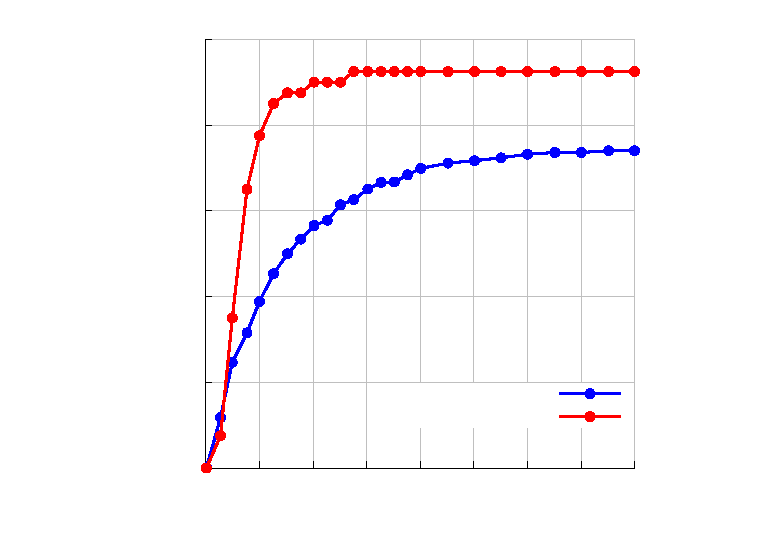
\includegraphics{distThreshVsAccuracy-s10e/distThreshVsAccuracy-s10e}}%
    \gplfronttext
  \end{picture}%
\endgroup

	\caption[Translation error threshold vs accuracy on s10e query set]{Comparison between InLoc and InLocCIIRC on their respective datasets. The s10e query set was used for InLocCIIRC. The independent variable describes the maximum allowed translation error. The angular threshold is set to $10\degree$.}
	\label{fig:dist-thresh-vs-accuracy}
\end{figure}

Figures \ref{fig:topView-B-315} and \ref{fig:topView-B-670} depict the dataset including the localization results.

\begin{figure}[htb!]
	\centering
 	\includegraphics[width=0.79\textwidth]{evaluation-s10e/topView-B-315}
 	\caption[s10e B-315 top-view]{View on the floor plan of room B-315. Red dots: sweeps. Blue dots: queries. Yellow dots: estimated query poses. The s10e query set was used.}
 	\label{fig:topView-B-315}
\end{figure} 

\begin{figure}[htb!]
	\centering
 	\includegraphics[width=0.69\textwidth]{evaluation-s10e/topView-B-670}
 	\caption[s10e B-670 top-view]{View on the floor plan of room B-670. Red dots: sweeps. Blue dots: queries. Yellow dots: estimated query poses. No s10e queries were incorrectly localized to this room.}
 	\label{fig:topView-B-670}
\end{figure} 

\section{HoloLens1 query set}

\subsection{Summary}

\begin{table}[htb!]
	\centering
	\rowcolors{2}{gray!20}{}
	\begin{tabular}{|c|c|c|c|}
		\hline
		\diagbox{\small Method}{\small Threshold} & 0.25m & 0.50m & 1.00m \\
		\hline
		k=1 (non-sequential) & 63.80\% & 81.90\% & 85.89\% \\
		\hline
		sequentialPV, k=2 & 63.80\% & 82.52\% & 86.50\% \\
		\hline
		sequentialPV, k=3 & 63.80\% & 83.44\% & 86.50\% \\
		\hline
		sequentialPV, k=4 & 61.96\% & 82.52\% & 85.28\% \\
		\hline
		MultiCameraPose, k=2 & \bfseries 68.41\% & \bfseries 83.74\% & \bfseries 87.12\% \\
		\hline
		MultiCameraPose, k=3 & \bfseries 68.41\% & 81.60\% & 86.20\% \\
		\hline
		MultiCameraPose, k=5 & 67.18\% & 80.67\% & 85.58\% \\
		\hline
		\bfseries HoloLens & \bfseries 84.36\% & \bfseries 97.55\% & \bfseries 97.55\% \\
		\hline
	\end{tabular}
	\caption[InLocCIIRC performance on HoloLens1 query set]{Evaluation of performance of localization methods on HoloLens1 query set (part of the InLocCIIRC dataset). Percentage rate of correctly localized queries within given threshold is shown. Angular threshold is equal to $10\degree$ in every row. The HoloLens method are the poses provided by HoloLens tracking itself, after being converted to be wrt World coordinate system. As it can be seen, it is superior to all the custom methods I have tried.}
	\label{tab:HL1-InLoc-statistics}
\end{table}

\begin{table}[htb!]
	\centering
	\rowcolors{2}{gray!20}{}
	\begin{tabular}{|c|c|c|c|c|c|c|}
		\hline
		\diagbox{\small Method}{\small Statistics} & \multicolumn{2}{c|}{Mean} & \multicolumn{2}{c|}{Median} & \multicolumn{2}{c|}{Std} \\
		\hline
		k=1 & 0.52m & 3.62$\degree$ & 0.18m & 2.01$\degree$ & 1.64m & 11.33$\degree$ \\
		\hline
		sequentialPV, k=2 & 0.52m & 3.05$\degree$ & 0.17m & 2.06$\degree$ & 1.64m & 5.21$\degree$ \\
		\hline
		sequentialPV, k=3 & \bfseries 0.45m & 3.04$\degree$ & 0.18m & 2.02$\degree$ & \bfseries 1.36m & 5.21$\degree$ \\
		\hline
		sequentialPV, k=4 & 0.60m & 3.61$\degree$ & 0.19m & 2.02$\degree$ & 1.93m & 11.47$\degree$ \\
		\hline
		MCP, k=2 & 0.53m & 2.76$\degree$ & \bfseries 0.16m & \bfseries 1.85$\degree$ & 1.84m & 4.41$\degree$ \\
		\hline
		MCP, k=3 & 0.54m & \bfseries 2.68$\degree$ & \bfseries 0.16m & 1.99$\degree$ & 1.85m & \bfseries 3.06$\degree$ \\
		\hline
		MCP, k=5 & 0.60m & 3.59$\degree$ & 0.17m & 2.02$\degree$ & 1.92m & 11.26$\degree$ \\
		\hline
		\bfseries HoloLens & \bfseries 0.15m & \bfseries 2.09$\degree$ & \bfseries 0.14m & \bfseries 1.51$\degree$ & \bfseries 0.08m & \bfseries 1.69$\degree$ \\
		\hline
	\end{tabular}
	\caption[HoloLens1 pose estimation error statistics]{Statistics of the HoloLens1 pose estimation errors. InLocCIIRC got completely lost 29 out of 350 times for all methods (except the HoloLens method). The HoloLens method got completely lost 6 out of 350 times, which is caused by the HoloLens delay (see table \ref{tab:HL-pose-delays}). The \emph{completely lost} cases are not included in the mean/median/std errors. Errors are computed by comparing InLocCIIRC pose estimates (or the pose estimates from HoloLens converted to be wrt World CS) with reference poses. The errors in [m] units are translation errors and the errors in [$\degree$] units are orientation errors. Lowest errors are highlighted in bold. MCP stands for MultiCameraPose. The original HoloLens method is superior to all the custom methods I have tried. Note that if the estimated poses were compared to the (unknown) ground-truth poses, the errors would likely be even lower, as discussed in the Reference poses section \ref{paragraph:gt-vs-ref-poses}.}
	\label{tab:HL1-other-statistics}
\end{table}

\subsection{Best custom method}

Judging from the results above, the best performing custom method is MultiCameraPose with sequence length $k=2$. 

\begin{figure}[htb!]
	\centering
	% GNUPLOT: LaTeX picture with Postscript
\begingroup
  \makeatletter
  \providecommand\color[2][]{%
    \GenericError{(gnuplot) \space\space\space\@spaces}{%
      Package color not loaded in conjunction with
      terminal option `colourtext'%
    }{See the gnuplot documentation for explanation.%
    }{Either use 'blacktext' in gnuplot or load the package
      color.sty in LaTeX.}%
    \renewcommand\color[2][]{}%
  }%
  \providecommand\includegraphics[2][]{%
    \GenericError{(gnuplot) \space\space\space\@spaces}{%
      Package graphicx or graphics not loaded%
    }{See the gnuplot documentation for explanation.%
    }{The gnuplot epslatex terminal needs graphicx.sty or graphics.sty.}%
    \renewcommand\includegraphics[2][]{}%
  }%
  \providecommand\rotatebox[2]{#2}%
  \@ifundefined{ifGPcolor}{%
    \newif\ifGPcolor
    \GPcolorfalse
  }{}%
  \@ifundefined{ifGPblacktext}{%
    \newif\ifGPblacktext
    \GPblacktexttrue
  }{}%
  % define a \g@addto@macro without @ in the name:
  \let\gplgaddtomacro\g@addto@macro
  % define empty templates for all commands taking text:
  \gdef\gplbacktext{}%
  \gdef\gplfronttext{}%
  \makeatother
  \ifGPblacktext
    % no textcolor at all
    \def\colorrgb#1{}%
    \def\colorgray#1{}%
  \else
    % gray or color?
    \ifGPcolor
      \def\colorrgb#1{\color[rgb]{#1}}%
      \def\colorgray#1{\color[gray]{#1}}%
      \expandafter\def\csname LTw\endcsname{\color{white}}%
      \expandafter\def\csname LTb\endcsname{\color{black}}%
      \expandafter\def\csname LTa\endcsname{\color{black}}%
      \expandafter\def\csname LT0\endcsname{\color[rgb]{1,0,0}}%
      \expandafter\def\csname LT1\endcsname{\color[rgb]{0,1,0}}%
      \expandafter\def\csname LT2\endcsname{\color[rgb]{0,0,1}}%
      \expandafter\def\csname LT3\endcsname{\color[rgb]{1,0,1}}%
      \expandafter\def\csname LT4\endcsname{\color[rgb]{0,1,1}}%
      \expandafter\def\csname LT5\endcsname{\color[rgb]{1,1,0}}%
      \expandafter\def\csname LT6\endcsname{\color[rgb]{0,0,0}}%
      \expandafter\def\csname LT7\endcsname{\color[rgb]{1,0.3,0}}%
      \expandafter\def\csname LT8\endcsname{\color[rgb]{0.5,0.5,0.5}}%
    \else
      % gray
      \def\colorrgb#1{\color{black}}%
      \def\colorgray#1{\color[gray]{#1}}%
      \expandafter\def\csname LTw\endcsname{\color{white}}%
      \expandafter\def\csname LTb\endcsname{\color{black}}%
      \expandafter\def\csname LTa\endcsname{\color{black}}%
      \expandafter\def\csname LT0\endcsname{\color{black}}%
      \expandafter\def\csname LT1\endcsname{\color{black}}%
      \expandafter\def\csname LT2\endcsname{\color{black}}%
      \expandafter\def\csname LT3\endcsname{\color{black}}%
      \expandafter\def\csname LT4\endcsname{\color{black}}%
      \expandafter\def\csname LT5\endcsname{\color{black}}%
      \expandafter\def\csname LT6\endcsname{\color{black}}%
      \expandafter\def\csname LT7\endcsname{\color{black}}%
      \expandafter\def\csname LT8\endcsname{\color{black}}%
    \fi
  \fi
    \setlength{\unitlength}{0.0500bp}%
    \ifx\gptboxheight\undefined%
      \newlength{\gptboxheight}%
      \newlength{\gptboxwidth}%
      \newsavebox{\gptboxtext}%
    \fi%
    \setlength{\fboxrule}{0.5pt}%
    \setlength{\fboxsep}{1pt}%
\begin{picture}(7200.00,5040.00)%
    \gplgaddtomacro\gplbacktext{%
      \csname LTb\endcsname%%
      \put(1685,704){\makebox(0,0)[r]{\strut{}$0$}}%
      \csname LTb\endcsname%%
      \put(1685,1527){\makebox(0,0)[r]{\strut{}$20$}}%
      \csname LTb\endcsname%%
      \put(1685,2350){\makebox(0,0)[r]{\strut{}$40$}}%
      \csname LTb\endcsname%%
      \put(1685,3173){\makebox(0,0)[r]{\strut{}$60$}}%
      \csname LTb\endcsname%%
      \put(1685,3996){\makebox(0,0)[r]{\strut{}$80$}}%
      \csname LTb\endcsname%%
      \put(1685,4819){\makebox(0,0)[r]{\strut{}$100$}}%
      \csname LTb\endcsname%%
      \put(1817,484){\makebox(0,0){\strut{}$0$}}%
      \csname LTb\endcsname%%
      \put(2331,484){\makebox(0,0){\strut{}$0.25$}}%
      \csname LTb\endcsname%%
      \put(2846,484){\makebox(0,0){\strut{}$0.5$}}%
      \csname LTb\endcsname%%
      \put(3360,484){\makebox(0,0){\strut{}$0.75$}}%
      \csname LTb\endcsname%%
      \put(3875,484){\makebox(0,0){\strut{}$1$}}%
      \csname LTb\endcsname%%
      \put(4389,484){\makebox(0,0){\strut{}$1.25$}}%
      \csname LTb\endcsname%%
      \put(4903,484){\makebox(0,0){\strut{}$1.5$}}%
      \csname LTb\endcsname%%
      \put(5418,484){\makebox(0,0){\strut{}$1.75$}}%
      \csname LTb\endcsname%%
      \put(5932,484){\makebox(0,0){\strut{}$2$}}%
    }%
    \gplgaddtomacro\gplfronttext{%
      \csname LTb\endcsname%%
      \put(1080,2761){\rotatebox{-270}{\makebox(0,0){\strut{}Correctly localized queries [\%]}}}%
      \put(3874,154){\makebox(0,0){\strut{}Distance threshold [meters]}}%
      \csname LTb\endcsname%%
      \put(5077,3063){\makebox(0,0)[r]{\strut{}k1}}%
      \csname LTb\endcsname%%
      \put(5077,2843){\makebox(0,0)[r]{\strut{}k2-MCP}}%
      \csname LTb\endcsname%%
      \put(5077,2623){\makebox(0,0)[r]{\strut{}HoloLens}}%
    }%
    \gplbacktext
    \put(0,0){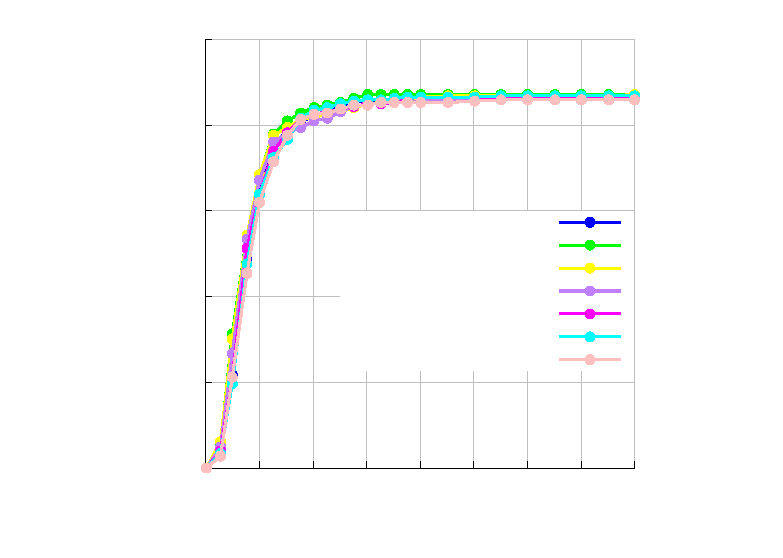
\includegraphics{distThreshVsAccuracy-HL1/distThreshVsAccuracy-HL1}}%
    \gplfronttext
  \end{picture}%
\endgroup

	\caption[Translation error threshold vs accuracy on HoloLens1 query set]{Evaluation of methods on the HoloLens1 query set. Comparison between the baseline method ($k=1$, i.e. non-sequential) with the best performing custom method ($k=2$, MultiCameraPose). The original HoloLens method, that we are aiming to surpass is also shown. The independent variable describes the maximum allowed translation error. The angular threshold is set to $10\degree$.}
	\label{fig:HL1-dist-thresh-vs-accuracy}
\end{figure}

{
\newcommand{\thiswidth}{0.26\linewidth} 
\setlength{\tabcolsep}{1pt}
\cellspacetoplimit 2pt
\cellspacebottomlimit 2pt
\begin{figure*}[htb!]
    \centering
    {\footnotesize
	\begin{tabular}{Sc|Sc|Sc|Sc|}
	& Query image & Closest cutout & Synthesized view \\
	\hline
	\makecell{Query 37 \\ OffMap \\ 0.05 m, 2.64$\degree$} &
    \adjincludegraphics[valign=M,width=\thiswidth]{evaluation-HL1-v4.2-k2/queryPipeline/PV/37.jpg/37.jpg/query_37} &
	\adjincludegraphics[valign=M,width=\thiswidth]{evaluation-HL1-v4.2-k2/queryPipeline/PV/37.jpg/37.jpg/chosen_cutout_B-315_1_-30_0} &
    \adjincludegraphics[valign=M,width=\thiswidth]{evaluation-HL1-v4.2-k2/queryPipeline/PV/37.jpg/37.jpg/synthesized_PV} \\
	%\adjincludegraphics[valign=M,width=\thiswidth]{evaluation-HL1-v4.2-k2/queryPipeline/PV/37.jpg/37.jpg/errmap} \\
	\hline
	\makecell{Query 57 \\ InMap \\ 0.17 m, 2.23$\degree$} &
    \adjincludegraphics[valign=M,width=\thiswidth]{evaluation-HL1-v4.2-k2/queryPipeline/PV/57.jpg/57.jpg/query_57} &
    \adjincludegraphics[valign=M,width=\thiswidth]{evaluation-HL1-v4.2-k2/queryPipeline/PV/57.jpg/57.jpg/chosen_cutout_B-315_2_-60_0} &
    \adjincludegraphics[valign=M,width=\thiswidth]{evaluation-HL1-v4.2-k2/queryPipeline/PV/57.jpg/57.jpg/synthesized_PV} \\
	%\adjincludegraphics[valign=M,width=\thiswidth]{evaluation-HL1-v4.2-k2/queryPipeline/PV/57.jpg/57.jpg/errmap} \\
	\hline
	\makecell{Query 84 \\ InMap \\ 12.18 m, 0.29$\degree$} &
    \adjincludegraphics[valign=M,width=\thiswidth]{evaluation-HL1-v4.2-k2/queryPipeline/PV/84.jpg/84.jpg/query_84} &
    \adjincludegraphics[valign=M,width=\thiswidth]{evaluation-HL1-v4.2-k2/queryPipeline/PV/84.jpg/84.jpg/chosen_cutout_B-315_19_-30_0} &
    \adjincludegraphics[valign=M,width=\thiswidth]{evaluation-HL1-v4.2-k2/queryPipeline/PV/84.jpg/84.jpg/synthesized_PV} \\
	%\adjincludegraphics[valign=M,width=\thiswidth]{evaluation-HL1-v4.2-k2/queryPipeline/PV/84.jpg/84.jpg/errmap} \\
	\hline
	\makecell{Query 155 \\ OffMap \\ 0.17 m, 0.70$\degree$} &
    \adjincludegraphics[valign=M,width=\thiswidth]{evaluation-HL1-v4.2-k2/queryPipeline/PV/155.jpg/155.jpg/query_155} &
    \adjincludegraphics[valign=M,width=\thiswidth]{evaluation-HL1-v4.2-k2/queryPipeline/PV/155.jpg/155.jpg/chosen_cutout_B-315_6_60_0} &
    \adjincludegraphics[valign=M,width=\thiswidth]{evaluation-HL1-v4.2-k2/queryPipeline/PV/155.jpg/155.jpg/synthesized_PV} \\
	%\adjincludegraphics[valign=M,width=\thiswidth]{evaluation-HL1-v4.2-k2/queryPipeline/PV/155.jpg/155.jpg/errmap} \\
	\hline
	\makecell{Query 206 \\ OffMap \\ 0.15 m, 0.80$\degree$} &
    \adjincludegraphics[valign=M,width=\thiswidth]{evaluation-HL1-v4.2-k2/queryPipeline/PV/206.jpg/206.jpg/query_206} &
    \adjincludegraphics[valign=M,width=\thiswidth]{evaluation-HL1-v4.2-k2/queryPipeline/PV/206.jpg/206.jpg/chosen_cutout_B-315_10_30_30} &
    \adjincludegraphics[valign=M,width=\thiswidth]{evaluation-HL1-v4.2-k2/queryPipeline/PV/206.jpg/206.jpg/synthesized_PV} \\
	%\adjincludegraphics[valign=M,width=\thiswidth]{evaluation-HL1-v4.2-k2/queryPipeline/PV/206.jpg/206.jpg/errmap} \\
	\hline
	\makecell{Query 322 \\ OffMap \\ 0.69 m, 3.41$\degree$} &
    \adjincludegraphics[valign=M,width=\thiswidth]{evaluation-HL1-v4.2-k2/queryPipeline/PV/322.jpg/322.jpg/query_322} &
    \adjincludegraphics[valign=M,width=\thiswidth]{evaluation-HL1-v4.2-k2/queryPipeline/PV/322.jpg/322.jpg/chosen_cutout_B-315_2_-90_0} &
    \adjincludegraphics[valign=M,width=\thiswidth]{evaluation-HL1-v4.2-k2/queryPipeline/PV/322.jpg/322.jpg/synthesized_PV} \\
	%\adjincludegraphics[valign=M,width=\thiswidth]{evaluation-HL1-v4.2-k2/queryPipeline/PV/322.jpg/322.jpg/errmap} \\
	\hline
    \end{tabular}
    \caption[HoloLens1 query pipeline]{{\bf Qualitative comparison of HoloLens1 queries localization.} From left to right: Query name and localization error (meters, degrees), query image, the best matching database image, synthesized view at the estimated pose, error map between the query image and the synthesized view. Green dots are the inlier matches obtained by geometric verification. The pose estimation of query 84 is not completely wrong by human standards. InLocCIIRC matched the query image with a very similar cutout image, that is, however, at another location. Although this query is InMap, the chosen cutout is not the one that forms the InMap propery. Note that the query images have a different aspect ratio than the cutout images. The error maps not shown to save space.}
    \label{fig:HL1-queryPipeline}
    }
\end{figure*}
}

Figure \ref{fig:HL1-topView-B-315} depicts the top-view of B-315 including a subset of localization results (every 20th HoloLens query is rendered). View of room B-670 is not shown, as for this subset of results, it looks the same as in case of s10e query set, see figure \ref{fig:topView-B-670}. This means that none of the queries in the subset were incorrectly localized in room B-670.

\begin{figure}[htb!]
	\centering
 	\includegraphics[width=0.80\textwidth]{evaluation-HL1-v4.2-k2/topView-B-315}
 	\caption[HoloLens1 B-315 top-view]{View on the floor plan of room B-315. Red dots: sweeps. Blue dots: queries. Yellow dots: estimated query poses. Every 20th HoloLens1 query rendered.}
 	\label{fig:HL1-topView-B-315}
\end{figure} 

\section{Sources of errors}
\label{section:sources-of-errors}

\subsection{Previous queries have meaningful correspondences but current query does not have any correspondences}
\emph{This was observed on MultiCameraPose, k=2 experiment}. This results in InLocCIIRC completely being lost (returning \code{NaN} estimated pose), thus limiting the number of correctly localized queries given translation/orientation thresholds. In this scenario, the queries in the segment prior to the current query being processed have 2D-3D correspondences (found using geometric verification). Furthermore, those queries look meaningful upon manual inspection. However, we are interested in the current query, which does not have any correspondences. \code{MultiCameraPose} does not support a rig containing a camera for which there are no correspondences. Of course, we cannot use P3P on the current query, without knowing the query-cutout correspondences. Potential solution to this problem is: use the last estimated non-\code{NaN} pose in a sequence of queries ending with the current query. Limit the number as to how far into history to go. I did not have time to implement it. Known affected queries in HoloLens1 query set: 88, 122, 148, 231, 233, 236, 315, 319, 341. Why did we find no correspondences at those affected queries? For query 122 it is understandable - there was a very fast movement. For query 174 - it is somehow difficult, even the preceding queries 170-173 were hard to estimate (resulting poses were not \code{NaN}, but the errors from reference poses were high). However, for some affected queries, namely query 88, 148 and 231, a problem was discovered. The next subsection describes the problem.

\subsection{Bad input \code{score} matrix}
\emph{This was observed on non-sequential (k=1) and MultiCameraPose, k=2 experiments}. Known affected queries: 88, 148, 231\footnote{This query is somewhat blurry, which may also have an impact.}. This issue probably affects more queries than is currently known by me. It causes no 2D-3D correspondences to be found. It is a problem, that currently causes \code{NaN} pose estimate for the affected queries. But it can also lower estimation accuracy for the successor queries, if the affected query is considered within its segment. This is because currently, P3P is used (non-sequential pose estimation), if some of the queries in a segment have no correspondences. For those 3 known affected queries, investigation revealed that the chosen cutout (i.e. the top one in pose verification output) from the previous query was not even considered in the top \topRetrieval{} cutouts in the pose estimation step. The reason the previous query's chosen cutout was picked is that the queries have not changed much during the two frames. The score for those cutouts was:

\begin{table}[htb!]
	\centering
	\begin{tabular}{|c|c|}
		\hline
		Query ID & Ranking of the previous query's chosen cutout \\
		\hline
		\hline
		88 & 714 \\
		\hline
		148 & 138 \\
		\hline
		231 & 518 \\
		\hline
	\end{tabular}
	\caption[Queries affected by inaccurate \code{score}]{The ranking after sorting all cutouts for a given query by highest score. Only top \topRetrieval{} make it to the pose estimation step, others are not considered. This suggests that the scores are not completely correct.}
	\label{tab:bad-scores-wrong-candidates}
\end{table}

\subsection{Hard to pick top \topPE{} combinations for non-trivial segments}
\label{subsection:hard-top-pick-top-combinations}
Geometric verification step chooses top \topGV{} cutouts for each query based on the highest number of inliers. The wrong ones would normally be filtered out by pose verification. However, if segments of length $k>1$ are used, the top \topPE{} combinations (representing the current segment) don't necessarily contain only the reasonable query-cutout pairs. This is because we are only choosing top \topPE{} combinations from $\topGV^k$ possible combinations\footnote{We are not talking about combinations in a mathematical sense, but rather as a way of expressing a number of possibilities.}. There is no easy solution to this problem. Making pose estimation return significantly more than top \topPE{} candidates for each query will have a performance impact, because the pose verification step is already time consuming.

\subsection{No HoloLens poses}
Due to the delay (see table \ref{tab:HL-pose-delays}), some of the queries by the end of the HoloLens1 and HoloLens2 sequences do not have a pose estimated from HoloLens. In such a case we have to resort to using standard P3P, which performs (on average) worse than MultiCameraPose. Hopefully the delay was only caused by the software extracting the data from HoloLens and the delay is not actually present in real use. If it is present, it is a problem as the techniques based on InLoc described in this paper would not work in real-time.

\subsection{Geometric verification fails}
\label{subsection:GV-fails}
Our approach produced a completely wrong pose estimate in Query 40 of the s10e query set. Upon debugging the issue, it turns out that there actually were several viable cutouts, similar to the query image. One would expect the correspondences to be found there. However, the geometric verification step (GV) found zero correspondences. This issue shall be investigated further.

\section{Computational complexity}
The redesigned and improved pose estimation pipeline is a fairly complex piece of software. It is hard to compute the asymptotic complexity of processing a query image or a set of query images. The computational requirements are missing from the InLoc paper \cite{taira2018inloc}. However, the authors mention the need for about 14 GB RAM in their experiment, to hold the image descriptors in memory.

Table \ref{tab:emperical-complexity} shows the processing times I have measured. They are not necessarily accurate, as sometimes, the experiment was re-run while keeping some previously computed data.

\begin{table}[htb!]
	\centering
	\begin{tabular}{|c|c|c|}
		\hline
		Experiment & Step & Processing time\\
		\hline
		\hline
		s10e & GPU & 11 min \\
		s10e & CPU & 1h 46 min \\
		\hline
		HoloLens1-k1 & GPU & 11 min \\
		HoloLens1-k1 & CPU & about 20 hours \\
		\hline
		HoloLens1-k5-MCP & GPU & 10 min \\
		HoloLens1-k5-MCP & CPU & about 48 hours \\
		\hline
		HoloLens1-k4-sequentialPV & GPU & 5 min \\
		HoloLens1-k4-sequentialPV & CPU & about 40 hours \\
		\hline
	\end{tabular}
	\caption[Processing times of the experiments]{The experiment is split into two parts; the first part runs on a GPU (feature extraction) and the rest runs on a CPU. For the CPU instance, a machine with 45 threads and K8 2000 CPUs (or similar) was used. GPU instance used a single NVIDIA 1080Ti GPU with 8 threads. The processing time is a rough estimate.}
	\label{tab:emperical-complexity}
\end{table}

The preprocessing step shall also be taken into account. It takes about 20 minutes to create the \code{score} matrix for an s10e query set. It is done by executing \code{buildFeatures.m} followed by \code{buildScores.m}. The same task takes 22 minutes on the HoloLens1 query set. Note that both tasks share the same number of cutouts that require processing by \code{buildFeatures.m}.

The recommended amount of RAM for re-running the experiments is 90 GB.

\chapter{Conclusion}
\label{chapter:conclusion}

I have created a new dataset suitable for indoor visual localization; either on single RGB images or on a sequence of query images and localization data from HoloLens. I have adjusted the original\footnote{Original InLoc implementation available at \cite{InLocImplementation}.} InLoc implementation and made it work on the newly acquired dataset. The performance on the non-sequential s10e query set is very good (compared to results in InLoc paper). This is likely caused by the fact that our dataset is much smaller than the InLoc dataset. I have also implemented two novel methods that are based on InLoc \cite{taira2018inloc} - the sequentialPV method and the MultiCameraPose method. It was expected that the sequentialPV method would not to perform very well compared to HoloLens tracking. The MultiCameraPose method is more accurate than both the baseline InLoc method and the sequentialPV method. The resulting estimated poses are usable. However its performance is still significantly below the precision of HoloLens tracking itself. It is not clear why the new MultiCameraPose method is not performing that well. In the previous chapter, I have described known sources of errors, a lot of which can be targeted in a future work. This will certainly improve the evaluation performance.

\section{Future work}
Improve the accuracy of the MultiCameraPose method by fixing known sources of errors. Spend extra time to analyze why there are inaccurate poses for certain queries and suggest an enhancement. The work on the HoloLens2 sequence should be continued - we need to compute reference poses. The code is there, but currently we are missing more manually set-up 2D-3D correspondences. Also, the work on synthetic dataset generation using Habitat AI shall be continued. Although it cannot give us data from HoloLens tracking, it can be used to generate new indoor localization datasets, without the need for expensive equipment (such as a Matterport scanner). There are extra parameters such as setting up the cutout horizontal field of view, \code{dslevel}\footnote{Determines how much to downsample images in the pose verification step.}, \code{MultiCameraPose} software \cite{MultiCameraPose} parameters and more. The accuracy of the reference poses wrt ground truth poses shall be also improved.

The paper \cite{IsThisTheRightPlace} provides an improvement of the InLoc pose verification step. Once a reference implementation is available, I recommend incorporating the changes into our implementation.

The cutouts shall be regenerated with horizontal field of view equal to $60\degree$, to see if it improves performance. This hFoV would also match the InLoc cutouts' hFoV.

\appendix

\printindex

\appendix

%\bibliographystyle{amsalpha}
\bibliographystyle{iso690}
\bibliography{bibliography}

\end{document}